% -----------------------------------------------------------------------------
%       Centro Federal de Educação Tecnológica de Minas Gerais - CEFET-MG
%
%   Modelo de trabalho acadêmico monográfico de acordo com as normas da ABNT
%   (Tese de Doutorado, Dissertação de Mestrado ou Projeto de Qualificação)
%
%     Projeto hospedado em: https://github.com/cfgnunes/latex-cefetmg
%
%    Autores: Cristiano Fraga G. Nunes <cfgnunes@gmail.com>
%             Henrique E. Borges <henrique@lsi.cefetmg.br>
%             Denise de Souza <densouza@gmail.com>
%             Lauro César <https://code.google.com/p/abntex2/>
%
% -----------------------------------------------------------------------------

\documentclass[%
    %twoside,                   % Impressão em frente (anverso) e verso
    oneside,                    % Impressão apenas no anverso
]{cefetmg}

\usepackage[%
    alf,
    abnt-emphasize=bf,
    bibjustif,
    recuo=0cm,
    abnt-doi=expand,            % Expande um endereço iniciado com doi: para http://dx.doi.org/
    abnt-url-package=url,       % Utiliza o pacote url
    abnt-refinfo=yes,           % Utiliza o estilo bibliográfico abnt-refinfo
    abnt-etal-cite=3,
    abnt-etal-list=3,
    abnt-thesis-year=final
]{abntex2cite}                  % Configura as citações bibliográficas conforme a norma ABNT

% -----------------------------------------------------------------------------
% Pacotes utilizados
% -----------------------------------------------------------------------------
\usepackage[utf8]{inputenc}                                 % Codificação do documento
\usepackage[T1]{fontenc}                                    % Seleção de código de fonte
\usepackage{booktabs}                                       % Réguas horizontais em tabelas
\usepackage{color, colortbl}                                % Controle das cores
\usepackage{float}                                          % Necessário para tabelas/figuras em ambiente multi-colunas
\usepackage{graphicx}                                       % Inclusão de gráficos e figuras
\usepackage{icomma}                                         % Uso de vírgulas em expressões matemáticas
\usepackage{indentfirst}                                    % Indenta o primeiro parágrafo de cada seção
\usepackage{microtype}                                      % Melhora a justificação do documento
\usepackage{multirow, array}                                % Permite tabelas com múltiplas linhas e colunas
\usepackage{subeqnarray}                                    % Permite subnumeração de equações
\usepackage{verbatim}                                       % Permite apresentar texto tal como escrito no documento, ainda que sejam comandos Latex
\usepackage{amsfonts, amssymb, amsmath}                     % Fontes e símbolos matemáticos
\usepackage[algoruled, portuguese]{algorithm2e}             % Permite escrever algoritmos em português
\usepackage[scaled]{helvet}                                 % Usa a fonte Helvetica
%\usepackage{times}                                         % Usa a fonte Times
%\usepackage{palatino}                                      % Usa a fonte Palatino
%\usepackage{lmodern}                                       % Usa a fonte Latin Modern
%\usepackage[bottom]{footmisc}                              % Mantém as notas de rodapé sempre na mesma posição
%\usepackage{ae, aecompl}                                   % Fontes de alta qualidade
%\usepackage{latexsym}                                      % Símbolos matemáticos
%\usepackage{lscape}                                        % Permite páginas em modo "paisagem"
%\usepackage{picinpar}                                      % Dispor imagens em parágrafos
%\usepackage{scalefnt}                                      % Permite redimensionar tamanho da fonte
%\usepackage{subfig}                                        % Posicionamento de figuras
%\usepackage{upgreek}                                       % Fonte letras gregas


% Redefine a fonte para uma fonte similar a Arial (fonte Helvetica)
\renewcommand*\familydefault{\sfdefault}

% -----------------------------------------------------------------------------
% Configurações de aparência do PDF final
% -----------------------------------------------------------------------------
\makeatletter
\hypersetup{%
    portuguese,
    colorlinks=true,            % true: "links" coloridos; false: "links" em caixas de texto
    linkcolor=blue,             % Define cor dos "links" internos
    citecolor=blue,             % Define cor dos "links" para as referências bibliográficas
    filecolor=blue,             % Define cor dos "links" para arquivos
    urlcolor=blue,              % Define a cor dos "hiperlinks"
    breaklinks=true,
    pdftitle={\@title},
    pdfauthor={\@author},
    pdfkeywords={abnt, latex, abntex, abntex2}
}
\makeatother

% Altera o aspecto da cor azul
\definecolor{blue}{RGB}{41,5,195}

% Redefinição de labels
\renewcommand{\algorithmautorefname}{Algoritmo}
\def\equationautorefname~#1\null{Equa\c c\~ao~(#1)\null}

% Cria o índice remissivo
\makeindex

% Hifenização de palavras que não estão no dicionário
\hyphenation{%
    qua-dros-cha-ve
    Kat-sa-gge-los
}

% -----------------------------------------------------------------------------
% Inclui os arquivos do trabalho acadêmico
% -----------------------------------------------------------------------------

% Insere e constrói alguns elementos pré-textuais para gerar capa, folha de rosto e folha de aprovação
% -----------------------------------------------------------------------------
% Capa
% -----------------------------------------------------------------------------

% -----------------------------------------------------------------------------
% ATENÇÃO:
% Caso algum campo não se aplique ao seu documento - por exemplo, em seu trabalho
% não houve coorientador - não comente o campo, apenas deixe vazio, assim: \campo{}
% -----------------------------------------------------------------------------

% -----------------------------------------------------------------------------
% Dados do trabalho acadêmico
% -----------------------------------------------------------------------------

\titulo{Simulação do funcionamento do modelo de protocolos TCP/IP}
%\title{Title in English}
\subtitulo{}
\autor{Thais Diniz Braz}
\local{Belo Horizonte}
\data{Junho de 2016} % Normalmente se usa apenas mês e ano

% -----------------------------------------------------------------------------
% Natureza do trabalho acadêmico
% Use apenas uma das opções: Tese (p/ Doutorado), Dissertação (p/ Mestrado) ou
% Projeto de Qualificação (p/ Mestrado ou Doutorado), Trabalho de Conclusão de
% Curso (Graduação)
% -----------------------------------------------------------------------------

\projeto{Projeto de Qualificação}

% -----------------------------------------------------------------------------
% Título acadêmico
% Use apenas uma das opções:
% - Se a natureza for Tese, coloque Doutor
% - Se a natureza for Dissertação, coloque Mestre
% - Se a natureza for Projeto de Qualificação, coloque Mestre ou Doutor conforme o caso
% - Se a natureza for Trabalho de Conclusão de Curso, coloque Bacharel
% -----------------------------------------------------------------------------

\tituloAcademico{Doutor}

% -----------------------------------------------------------------------------
% Área de concentração e linha de pesquisa
% OBS: indique o nome da área de concentração e da linha de pesquisa do Programa de Pós-graduação
% nas quais este trabalho se insere
% Se a natureza for Trabalho de Conclusão de Curso, deixe ambos os campos vazios
% -----------------------------------------------------------------------------

\areaconcentracao{}
\linhapesquisa{}

% -----------------------------------------------------------------------------
% Dados da instituição
% OBS: a logomarca da instituição deve ser colocada na mesma pasta que foi colocada o documento
% principal com o nome de "logoInstituicao". O formato pode ser: pdf, jpf, eps
% Se a natureza for Trabalho de Conclusão de Curso, coloque em "programa' o nome do curso de graduação
% -----------------------------------------------------------------------------

\instituicao{Centro Federal de Educação Tecnológica de Minas Gerais}
\programa{Engenharia da Computação}
%\programa{Curso de Engenharia de Computação}
\logoinstituicao{0.2}{./04-figuras/logo-instituicao.pdf} % \logoinstituicao{<escala>}{<nome do arquivo>}

% -----------------------------------------------------------------------------
% Dados do(s) orientador(es)
% -----------------------------------------------------------------------------

\orientador{Sandro Renato Dias}
%\orientador[Orientadora:]{Nome da orientadora}
\instOrientador{Centro Federal de Educação Tecnológica de Minas Gerais}

\coorientador{}
%\coorientador[Coorientadora:]{Nome da coorientadora}
\instCoorientador{}

%% -----------------------------------------------------------------------------
% Folha de Rosto
% -----------------------------------------------------------------------------

% Trabalho de Conclusão de Curso
%\preambulo{{\imprimirprojeto} apresentado ao Curso de Engenharia de Computação do Centro Federal de Educação Tecnológica de Minas Gerais, como requisito parcial para a obtenção do título de {\imprimirtituloAcademico} em Engenharia de Computação.}

% Projeto de qualificação de Mestrado ou Doutorado
\preambulo{{\imprimirprojeto} apresentado ao Programa de \mbox{Pós-graduação} em Modelagem Matemática e Computacional do Centro Federal de Educação Tecnológica de Minas Gerais, como requisito parcial para a obtenção do título de {\imprimirtituloAcademico} em Modelagem Matemática e Computacional.}

% Dissertação de Mestrado
%\preambulo{{\imprimirprojeto} apresentada ao Programa de \mbox{Pós-graduação} em Modelagem Matemática e Computacional do Centro Federal de Educação Tecnológica de Minas Gerais, como requisito parcial para a obtenção do título de {\imprimirtituloAcademico} em Modelagem Matemática e Computacional.}

% Tese de Doutorado
%\preambulo{{\imprimirprojeto} apresentada ao Programa de \mbox{Pós-graduação} em Modelagem Matemática e Computacional do Centro Federal de Educação Tecnológica de Minas Gerais, como requisito parcial para a obtenção do título de {\imprimirtituloAcademico} em Modelagem Matemática e Computacional.}

% -----------------------------------------------------------------------------
% Edite este arquivo comentando as linhas que não se aplicam ao tipo de documento acadêmico pretendido.
% -----------------------------------------------------------------------------

%% -----------------------------------------------------------------------------
% Folha de Aprovação
% -----------------------------------------------------------------------------

\textopadraofolhadeaprovacao{Esta folha deverá ser substituída pela cópia digitalizada da folha de aprovação fornecida.}

% -----------------------------------------------------------------------------
% Este documento foi mantido apenas para preservar a paginação do trabalho
% acadêmico final, após a inserção da folha de aprovação fornecida
% -----------------------------------------------------------------------------


\begin{document}

% Insere os elementos pré-textuais
\pretextual
\imprimircapa                                               % Comando para imprimir Capa
\imprimirfolhaderosto{}                                     % Comando para imprimir Folha de rosto
%\imprimirfolhadeaprovacao{}                                 % Comando para imprimir Folha de aprovação
%% -----------------------------------------------------------------------------
% Dedicatória
% -----------------------------------------------------------------------------

\begin{dedicatoria}

Edite este texto para inserir uma dedicatória que lhe convenha.

\end{dedicatoria}
           % Dedicatória
%% -----------------------------------------------------------------------------
% Agradecimentos
% -----------------------------------------------------------------------------

\begin{agradecimentos}

Edite e coloque aqui os agradecimentos às pessoas e/ou instituições que contribuíram para a realização do trabalho.

É obrigatório o agradecimento às instituições de fomento à pesquisa que financiaram total ou parcialmente o trabalho, inclusive no que diz respeito à concessão de bolsas.

\end{agradecimentos}
        % Agradecimentos
%% -----------------------------------------------------------------------------
% Epígrafe
% -----------------------------------------------------------------------------

\begin{epigrafe}

\textit{``Por mim se vai à cidade das dores; por mim se vai à ininterrupta dor [...]. Abandonai toda a esperança, ó vós que entrais!''}
(Dante Alighieri, p. 17, inscrição à porta do Inferno)

\end{epigrafe}

% -----------------------------------------------------------------------------
% Edite o texto acima para inserir uma epígrafe de sua preferência
% -----------------------------------------------------------------------------
              % Epígrafe
%% -----------------------------------------------------------------------------
% Resumo
% -----------------------------------------------------------------------------

\begin{resumo}
    Síntese do trabalho em texto cursivo contendo um único parágrafo.
    Para uma Tese de Doutorado o resumo deve conter, no máximo, 500 palavras.
    Para uma Dissertação de Mestrado o resumo deve conter, no máximo, 250 palavras.
    Para um Projeto de Qualificação o resumo deve conter, no máximo, 200 palavras.
    O resumo é a apresentação clara, concisa e seletiva do trabalho.
    No resumo deve-se incluir, preferencialmente, nesta ordem:brevíssima introdução ao assunto do trabalho de pesquisa (incluindo motivação e justificativa para a realização deste trabalho), o que será feito no trabalho (objetivos), como ele será desenvolvido (metodologia), quais são os principais resultados obtidos ou esperados e a conclusão (compare os resultados com os da literatura e destaque as principais contribuições científicas do trabalho.

    \textbf{Palavras-chave}: Modelo Latex. Trabalho acadêmico monográfico. Normas ABNT. Outra palavra.
\end{resumo}

% -----------------------------------------------------------------------------
% Escolha de 3 a 6 palavras ou termos que descrevam bem o seu trabalho. As palavras-chaves são utilizadas para indexação.
% A letra inicial de cada palavra deve estar em maiúsculas. As palavras-chave são separadas por ponto.
% -----------------------------------------------------------------------------
             % Resumo na língua vernácula
%% -----------------------------------------------------------------------------
% Abstract
% -----------------------------------------------------------------------------

\begin{resumo}[Abstract]
    Translation of the abstract into english, possibly adapting or slightly changing the text in order to adjust it to the grammar of Standard English.
    Try to stay within the limit of: 500 word for a PhD Thesis;
    250 words for a Master Dissertation;
    200 words for a Qualifying Research Project.

    \textbf{Keywords}: Latex model. Academic work. ABNT standards. Another word.
\end{resumo}

% -----------------------------------------------------------------------------
% O restante da formatação deve manter-se igual ao do resumo em português, i.e, um único parágrafo.
% -----------------------------------------------------------------------------
             % Resumo em língua inglesa
% -----------------------------------------------------------------------------
% Lista de Figuras
% -----------------------------------------------------------------------------

\pdfbookmark[0]{\listfigurename}{lof}
\listoffigures*
\cleardoublepage

% -----------------------------------------------------------------------------
% Este arquivo não necessita de ser editado. A lista é gerada automaticamente.
% -----------------------------------------------------------------------------
         % Lista de figuras
%% -----------------------------------------------------------------------------
% Lista de Tabelas
% -----------------------------------------------------------------------------

\pdfbookmark[0]{\listtablename}{lot}
\listoftables*
\cleardoublepage

% -----------------------------------------------------------------------------
% Este arquivo não necessita de ser editado. A lista é gerada automaticamente.
% -----------------------------------------------------------------------------
         % Lista de tabelas
%% -----------------------------------------------------------------------------
% Lista de Quadros
% -----------------------------------------------------------------------------

\pdfbookmark[0]{\listofquadrosname}{loq}
\listofquadros*
\cleardoublepage

% -----------------------------------------------------------------------------
% Este arquivo não necessita de ser editado. A lista é gerada automaticamente.
% -----------------------------------------------------------------------------
         % Lista de quadros
%% -----------------------------------------------------------------------------
% Lista de Algoritmos
% -----------------------------------------------------------------------------

\newcommand{\algoritmoname}{Algoritmo}
\renewcommand{\listalgorithmcfname}{Lista de Algoritmos}

\floatname{algocf}{\algoritmoname}
\newlistof{listofalgoritmos}{loa}{\listalgoritmoname}
\newlistentry{algocf}{loa}{0}

\counterwithout{algocf}{chapter}
\renewcommand{\cftalgocfname}{\algoritmoname\space}
\renewcommand*{\cftalgocfaftersnum}{\hfill--\hfill}

\pdfbookmark[0]{\listalgorithmcfname}{loa}
\listofalgorithms
\cleardoublepage

% -----------------------------------------------------------------------------
% Este arquivo não necessita de ser editado. A lista é gerada automaticamente.
% -----------------------------------------------------------------------------
      % Lista de algoritmos
%% -----------------------------------------------------------------------------
% Lista de Siglas
% -----------------------------------------------------------------------------

\begin{siglas}
    \item[ABNT] Associação Brasileira de Normas Técnicas
    \item[DECOM] Departamento de Computação
\end{siglas}

% -----------------------------------------------------------------------------
% Edite a lista acima para definir "todos" os acrônimos e siglas utilizados neste trabalho
% -----------------------------------------------------------------------------
          % Lista de abreviaturas e siglas
%% -----------------------------------------------------------------------------
% Lista de Símbolos
% -----------------------------------------------------------------------------

\begin{simbolos}
    \item[$ \Gamma $] Letra grega Gama
    \item[$ \lambda $] Comprimento de onda
    \item[$ \in $] Pertence
\end{simbolos}

% -----------------------------------------------------------------------------
% Edite a lista acima para definir "todos" os símbolos utilizados neste trabalho
% -----------------------------------------------------------------------------
        % Lista de símbolos
% -----------------------------------------------------------------------------
% Sumário
% -----------------------------------------------------------------------------

\pdfbookmark[0]{\contentsname}{toc}
\tableofcontents*
\cleardoublepage

% -----------------------------------------------------------------------------
% Este arquivo não necessita de ser editado. O sumário é gerado automaticamente.
% -----------------------------------------------------------------------------
               % Sumário

% Insere os elementos textuais
\textual
% -----------------------------------------------------------------------------
% Introdução
% -----------------------------------------------------------------------------

\chapter{Introdução}
\label{chap:introducao}

A Internet está intrinsecamente presente na vida da sociedade contemporânea, de tal forma que as pessoas a consideram indispensável. Inseridos neste contexto, o modo de ter acesso ao mundo se adaptou: a obtenção de informações, comunicação, estudo, pesquisas, relacionamentos e etc. 

\citeonline{KUROSE} levantam a possibilidade da Internet ser o "maior sistema de engenharia já criado pela humanidade". Porém, apesar da Internet fazer parte da vida cotidiana de forma tão categórica, o primeiro contato, do ponto de vista do usuário doméstico, ocorreu apenas nos anos 90, pouco mais de 20 anos após o início do seu desenvolvimento.

Em 1967 foi apresentada, pela ARPA (\textit{Advanced Research Projects Agency}) do departamento de defesa dos Estados Unidos, a ARPANET. Idealizada como uma pequena rede de computadores conectados, no qual cada host (sistema final conectado à rede) fosse ligado à um computador especializado, denominado \textit{Interface Message Processor} (IMP), sendo que estes seriam conectados à outros IMPs. Esta ideia foi concretizada 2 anos depois e em 1969 o sistema começou a operar em quatro localidades distintas. As	 Universidades da California de Los Angeles e Santa Barbara (UCLA e UCSB, respectivamente), em conjunto com o Instituto de Pesquisa de Stanford (SRI) e com a Universidade de Utah foram conectados através de seus IMPs. Um software, chamado NCP (\textit{Network Control Protocol}), possibilitava a comunicação entre os institutos \cite{FOR}. Foi a primeira rede de comutação de pacotes operacional (os dados a serem transferidos através da rede são divididos em pequenas partes, multiplexadas em conexões entre máquinas) \cite{COMER}.

A partir do funcionamento bem sucedido da ARPANET, a mesma tecnologia de troca de pacotes foi empregado na comunicação por rádio tático e por satélite (SATNET). Porém, devido a particularidades de cada ambiente de comunicação, cada uma dessas redes utilizava diferentes parâmetros técnicos, foi necessário, ent\~ao a criação de protocolos para integrá-las \cite{STALLINGS}. Vincent Cerf e Bob Khan idealizaram, em 1972, um projeto de interligação de rede, chamado \textit{Internetting Project}, que pode ser considerado o predecessor da própria Internet. Para resolver os problemas de comunicação direta entre diferentes hosts, a solução sugerida foi a criação um hardware intermediário entre uma rede e outra, este dispositivo foi chamado \textit{gateway}.

Em 1974 foi publicado um artigo \cite{Cerf} no qual foi apresentado o protocolo TCP. A descrição presente no artigo original resume precisamente o conteúdo proposto: "Um protocolo que suporta o compartilhamento de recursos que existem em diferentes redes de comutação de pacotes. O protocolo prevê variação em tamanhos de pacotes de rede individuais, falhas de transmissão, sequenciamento, controle de fluxo, verificação de erros fim-a-fim, bem como a criação e destruição de conexões lógicas processo-a-processo".

De acordo com \citeonline{FOR}, pouco tempo depois as autoridades decidiram dividir o TCP em dois protocolos distintos, o TCP (\textit{Transmission Control Protocol}) e o IP (\textit{Internetworking Protocol}), e, em 1983, em detrimento dos protocolos originais da ARPANET, o TCP/IP tornou-se o modelo de conexão oficial da Internet. Ou seja, a partir de então, para se conectar à Internet, tornou-se necessário a execução deste modelo, o qual possibilita a intercomunicação entre redes heterogêneas, conectando, assim, milhares de dispositivos comunicantes de abrangência mundial.

O modelo de protocolo TCP/IP é definido oficialmente pelo IETF (\textit{Internet Engineering Task Force}), instituição que especifica os padrões que serão implementados e utilizados em toda a Internet, no RFC\footnote{\textit{Request for Comments}: Documentos mantidos pela IETF que contêm conteúdo técnico e organizacional sobre a Internet.} 1180 \cite{RFC1180}.

Pode-se perceber assim a importância do modelo TCP/IP, e, desta forma, surge a necessidade do seu estudo e entendimento por parte dos alunos de cursos que possuem em seu escopo o ensino de Redes de Computadores, como Engenharia da Computação e Elétrica, Sistemas de Informação, Ciência da Computação e etc. e consequentemente o conhecimento dos profissionais no mercado.

Dado tal contexto este trabalho se propôs, então, a partir da simulação do funcionamento do modelo de protocolos TCP/IP, formular um sistema a ser utilizado na aprendizagem, pretendendo compor a didática do ensino deste t\'opico na disciplina de Redes de Computadores, com o objetivo apoiar o docente no ensino e os alunos no aprendizado. Essa simulação é composta por quatro aplicações, cada uma simulando uma das camadas presentes na pilha de protocolos TCP/IP: aplicação, transporte, rede e física. Visando a exposição dos pacotes referentes a cada camada, e seu conteúdo. 

Está incluso no escopo do trabalho apenas os principais protocolos utilizados em cada camada e seus funcionamentos ideais. Futuramente pretende-se a inclusão de erros e tratamento destes, para aprofundar o aprendizado da lógica por trás das ações de cada protocolo.                 % Introdução
% -----------------------------------------------------------------------------
% Fundamentação Teórica
% -----------------------------------------------------------------------------

\chapter{Fundamentação Teórica}
\label{chap:fundamentacaoTeorica}

Os protocolos, anteriormente mencionados neste trabalho, são um conjunto de formalidades a serem seguidas para permitir a conversação e o entendimento entre dois dispositivos conectados à rede, chamados hosts. Nos modelos de conexão a serem apresentados (OSI e TCP/IP), estes protocolos são divididos em diferentes camadas para que assim os problemas possam ser tratados separadamente. Essa divisão se faz necessária devido à complexidade na comunicação. Além disso, este modelo provê a abstração de uma camada à sua respectiva camada superior.

Quando o dado é enviado de um host para outro, ele passa pelas várias camadas estruturadas ainda no remetente, as quais adicionam informações de forma incremental, as quais serão necessárias para seu envio ou entendimento por parte do host que irá receber este pacote, gerando assim uma nova PDU (\textit{Protocol data unit}) a cada camada. Ao chegar no host destino este dado passa novamente pela pilha, porém em sentido inverso, e cada camada retira, interpreta os dados enviados pela camada correspondente e repassa pacote resultante é para camada superior. Este funcionamento é mostrado na Figura \ref{fig:camadas}, onde as PDU's são representadas pelos elementos ao lado de cada camada, é possível perceber seu incremento e decremento nos hosts remetente e destinatário, respectivamente. 
Todo este processo é realizado por protocolos pertencentes à cada nível, assim cada camada conversa apenas com sua correspondente.

\begin{figure}[H]
	\centering
    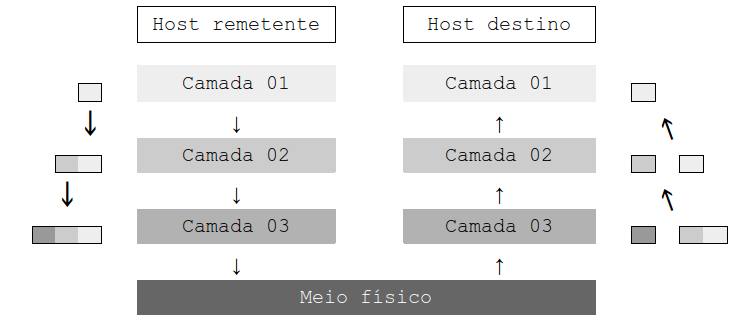
\includegraphics[width=\textwidth]{04-figuras/camadas.png}
    \caption{Funcionamento em camadas}
    \label{fig:camadas}
\end{figure}  	 
	 
	 
\section{Modelo de Referencia ISO OSI}

O modelo OSI (\textit{Open System Interconection}), Figura \ref{fig:OSI}, criado no final dos anos 70 pela ISO (\textit{International Sandards Organization}), é um modelo conceitual estruturado em camadas, que de acordo com \citeonline{FOR} aborda todos os aspectos da comunicação de rede. Este mesmo autor define o termo "Sistema Aberto" (termo presente no nome dado ao modelo), como um conjunto de protocolos os quais permitem a comunicação entre dois sistemas distintos, inclusive em suas arquiteturas. 

\begin{figure}[H]
	\centering
    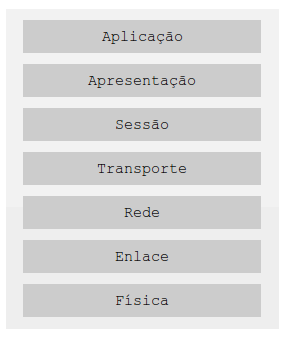
\includegraphics[width=0.5\textwidth]{04-figuras/OSI.png}
    \caption{Pilha do modelo de referência OSI}
    \fonte{\cite{COMER}}
    \label{fig:OSI}
\end{figure} 


Para que isto seja possível são necessárias camadas bem delimitadas e com fuç\~oes bem especificas: de acordo com \citeonline{STALLINGS}, limites bem definidos tornam possível que mudanças em uma camada não afetem os softwares existentes em outras camadas, já as restrições de suas funções provê o desenvolvimento independente de padrões.

%\citeonline{COMER} ressalta ainda que este modelo foi criado para descrever protocolos em uma única rede, assim diferentemente do modelo TCP/IP, não contem uma camada específica para encaminhamento de internet.



\section{Modelo TCP/IP}

A arquitetura do modelo TCP/IP é apresentada no RFC 1122 \cite{RFC1122}, o qual especifica os requerimentos exigidos para que um host seja capaz de se conectar à Internet. Este explana sobre as três últimas camadas do modelo: transporte, internet e enlace; já a primeira camada é apresentada separadamente pelo RFC 1123 \cite{RFC1123}.

%verify
Diferentemente do modelo ISO o conjunto de protocolos TCP/IP não são necessariamente interdependentes. Segundo \citeonline{FOR}, os protocolos presentes nesse modelo possuem uma certa autonomia e podem ser organizados de acordo com a necessidade da rede. O termo hierárquico apenas garante que um protocolo da camada superior seja suportado por outro(s) protocolo(s) da camada inferior.

\begin{figure}[H]
	\centering
    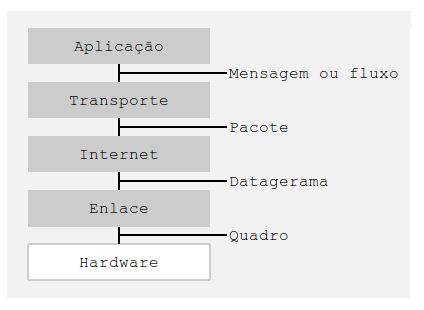
\includegraphics[width=0.65\textwidth]{04-figuras/TCPIP.png}
    \caption{Pilha do modelo TCP/IP e o nome das PDU's transferidas entre as camadas}
    \fonte{\cite{COMER}}
    \label{fig:TCPIP}
\end{figure} 

A Figura \ref{fig:TCPIP} representa a pilha do modelo TCP/IP e a nomenclatura referente aos pacotes, PDU's, transferidos entre cada camada. Complementarmente na Figura \ref{fig:relacao}, retirada do livro de \citeonline{FOR}, está representada a relação do modelo de camadas ISO e os protocolos pertencentes ao modelo TCP/IP. 

\begin{figure}[H]
	\centering
    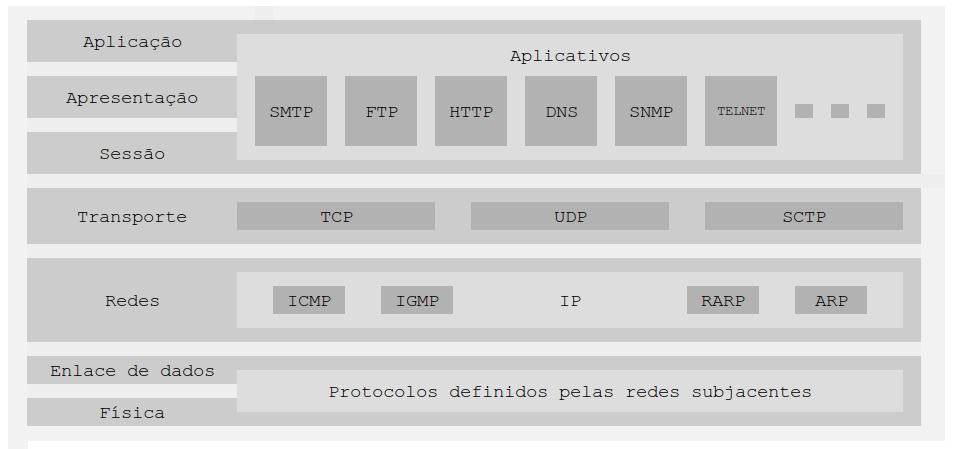
\includegraphics[width=\textwidth]{04-figuras/relacao.png}
    \caption{Relação entre o modelo de referência OSI e os protocolos pertencentes ao modelo TCP/IP }
    \label{fig:relacao}
    \fonte{\cite{FOR}}
\end{figure}    


Ademais é importante ressaltar que a maioria das literaturas que tratam deste assunto utilizam um modelo híbrido, entre o OSI e com TCP/IP. Este modelo apresenta 5 camadas e sua relação com o modelo original TCP/IP e o modelo OSI está representada na Figura \ref{fig:tresmodelos}. De acordo com \cite{TANENBAUM} esse modelo visa incluir os benefícios de ambas referências. Enquanto a separaç\~ao do modelo OSI e as definições caracter\'isticas de suas camadas ainda o torna desej\'avel como referência, o modelo TCP/IP contribui com seus protocolos amplamente aplicados.

\begin{figure}[H]
	\centering
    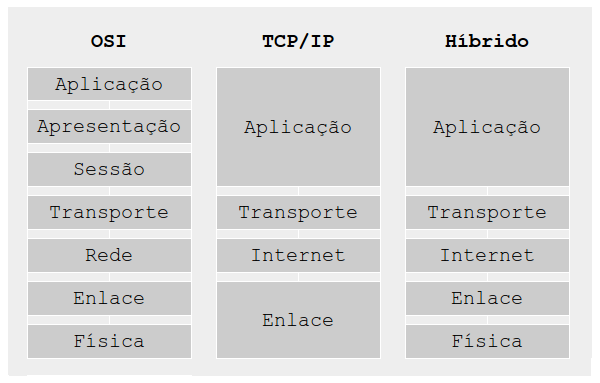
\includegraphics[width=0.75\textwidth]{04-figuras/tresmodelos.png}
    \caption{Relação entre o modelo de referencia OSI, o modelo de protocolos TCP/IP e o modelo híbrido}
    \label{fig:tresmodelos}
\end{figure} 

Neste trabalho iremos focar no modelo TCP/IP oficial, de quatro camadas, e seus protocolos, os quais serão apresentados nas subseções seguintes: 2.2.1 Aplicação, 2.2.2 Transporte, 2.2.3 Internet e 2.2.4 Enlace. 

\subsection{Aplicação}

Está é primeira camada da pilha TCP/IP, definida separadamente no RFC 1123 \cite{RFC1123}. Ela mantém protocolos necessários e utilizados pelos usuários e serviços. Em suma, aplicações de redes executadas em um sistema final tem o objetivo de se comunicar com outras aplicações em outro sistema conectado pela rede\cite{KUROSE}.

Os principais protocolos pertencentes à Aplicação, apresentados por \cite{STALLINGS}, são:
\begin{itemize}
\item Telnet: possibilita o usu\'ario acessar uma m\'aquina, atrav\'es de outro sistema.
\item FTP (\textit{File Transfer Protocol}): utilizado para transferir arquivos entre sistemas.
\item SMTP (\textit{Simple Mail Transfer Protocol}): prov\^e transporte de emails entre diferentes hosts.
\item HTTP (\textit{HyperText Transfer Protocol}): utilizado para a comunicação entre um sistema final e um servidor Web.
\item DNS (\textit{Domain Name System}): serviço de diretório que traduz nomes de hospedeiro para endereço IP.
\end{itemize}

Além de seus serviços é importante destacar as arquiteturas da camada de Aplicação. \citeonline{KUROSE} apresenta duas arquiteturas, as quais afirmam serem as mais comumente utilizadas hoje em dia, a cliente/servidor e a P2P(\textit{Peer to Peer}).

O autor explica que a arquitetura cliente/servidor é configurada em um sistemas finais: primeiramente é necessário que um host, chamado servidor, ofereça serviço através de uma rede, o qual será acessado por um ou mais host(s), denominado(s) cliente(s), que enviará uma requisição ao servidor e espera deste uma resposta. Para que isto seja poss\'ivel \'e necess\'ario que o hospedeiro que atua como servidor esteja sempre disponível, além de possuir um IP conhecido, ou o seu nome (neste caso o protocolo DNS precisa fazer a traduç\~ao).

A arquitetura P2P, é um pouco diferente, o mesmo autor explica que nesta configuração dois sistemas finais utilizam comunicação direta, sem a definição estrita de quem é cliente e quem é o servidor, sendo assim os hosts podem desempenhar ambas funções, de forma intercalada. Adicionando à estas arquiteturas, temos uma configuração híbrida, que utiliza inicialmente o cliente/servidor para estabelecer uma nova conexão entre diferentes hosts, que passam a se comunicar utilizando a arquitetura P2P.

\subsection{Transporte}

De acordo com \citeonline{TANENBAUM}, o objetivo desta camada é prover serviço de comunicação entre processos de aplicações, em diferentes sistemas finais, ou seja ampliar o serviço de entrega IP ( que será apresentado na próxima subseção) para um serviço de entrega entre dois processos que rodam nestes sistemas. Este tipo de comunicação é chamada transferência fim-a-fim.

O pacote de dados, PDU, pertencente à esta camada é chamado "seguimento", o qual contém informações referentes à camada de aplicação, e após ter inserido informaç\~oes adicionais, como aplicaç\~ao origem e destino e checksum (c\'odigo utilizado para a verificaç\~ao da integridade do pacote), a PDU é passada para camada seguinte, a de Rede.

A Internet possui dois protocolos distintos responsáveis pelo serviço de transporte, o TCP (\textit{Transmission Control Protocol}) e o UDP (\textit{User Datagram Protocol}). A principal diferença entre os protocolos citados é em relação à sua confiabilidade. O protocolo UDP fornece à camada de aplicação um serviço não confiável e orientado à mensagem, ao contrário do TCP, o qual garante uma transmissão confiável dos dados, utilizando para isso um serviço orientado à conexão, \cite{COMER}.

As principais características do protocolo TCP são apresentadas por \citeonline{KUROSE}, em seu texto eles explicam que para garantir uma entrega de dados correta e em ordem, entre processos remetente e destinatário, o protocolo TCP utiliza o controle de fluxo, números de sequência, reconhecimentos e temporizadores. Além de oferecer um serviço de controle de congestionamento, o qual limita a taxa de envio de tráfego do remetente para rede, permitindo que conexões TCP's compartilhem igualitariamente a largura de banda em um enlace de dados congestionado.

\begin{figure}[H]
	\centering
    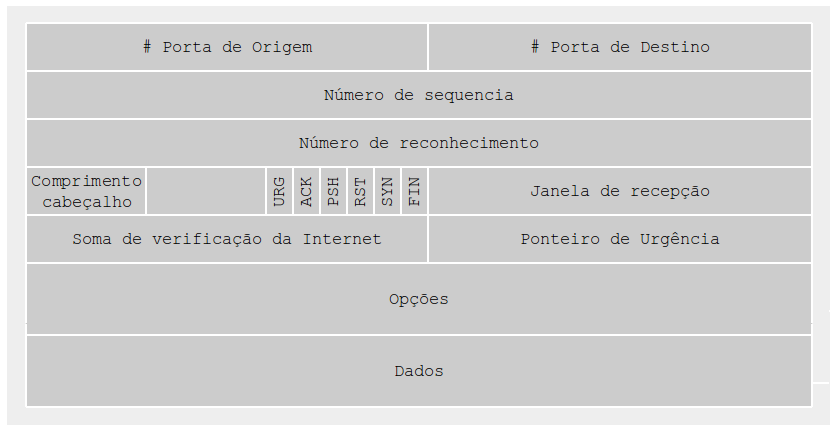
\includegraphics[width=\textwidth]{04-figuras/TCP.png}
    \caption{Estrutura da PDU do protocolo TCP}
    \label{fig:TCP}
    \fonte{\cite{KUROSE}}
\end{figure}

O mesmo autor afirma que o protocolo UDP \cite{RFC768}, entretanto, faz o mínimo necessário para a entrega de dados de uma aplicação à outra, este adiciona aos dados da camada de Aplicação apenas informações básicas para o encapsulamento da PDU em um segmento (chamado Datagrama). É possível reparar a diferença quanto a simplicidade da estrutura do segmento do protocolo UDP, apresentado na Figura \ref{fig:UDP}, em comparação com a estrutura do segmento do protocolo TCP, mostrado na Figura \ref{fig:TCP}.

\begin{figure}
	\centering
    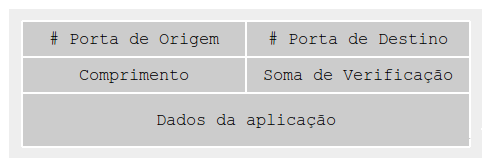
\includegraphics[width=0.75\textwidth]{04-figuras/UDP.png}
    \caption{Estrutura da PDU do protocolo UDP}
    \label{fig:UDP}
    \fonte{\cite{KUROSE}}
\end{figure}

As diferenças ressaltadas entre os protocolos TCP e UDP os tornam desejáveis para diferentes objetivos. Para conexões que são capazes de suportar perda de dados, como telefonia por Internet, ou necessitam de velocidade, como o protocolo DNS, é preferível a utilização do protocolo UDP. Já para os serviços que não suportam perdas e necessitam de confiabilidade, como HTTP, FTP e SMTP, o protocolo TCP é necessário.

Além dos protocolos citados, que são os mais conhecidos, \citeonline{FOR} citam outro protocolo pertencente a esta camada, o SCTP (\textit{Stream Control Transmission Protocol}), definido no RFC 4960 \cite{RFC4960}, que combina os melhores recursos dos protocolos TCP e UDP, assim ele provê um serviço confiável e orientado à mensagem.


\subsection{Rede}

Esta camada, também é chamada de internet (minúsculo para referenciar uma conexão de redes genérica), recebe o segmento enviado pela camada superior, de Transporte, juntamente com uma identificação do host para qual deve ser enviado este pacote, que então é encapsulado em um pacote IP (Figura \ref{fig:IP}) antes de ser repassado para camada seguinte \cite{COMER}.Todos os pacotes transportados pela rede devem possuir o endereço de destino completo, contendo o número IP, pois estes serão independentemente transportados. 

\begin{figure}[H]
	\centering
    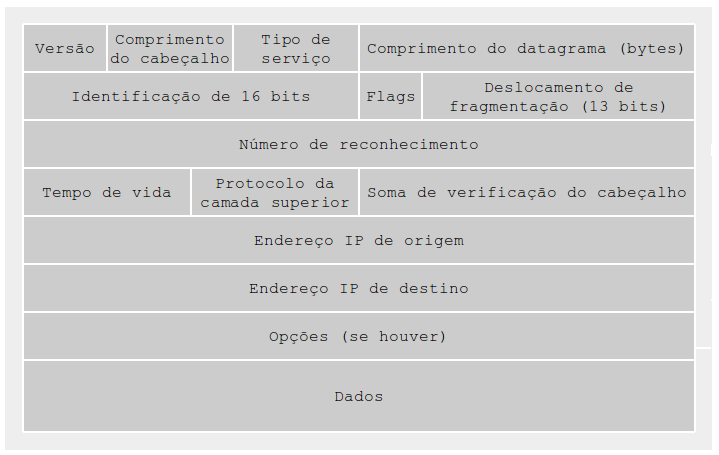
\includegraphics[width=\textwidth]{04-figuras/IPV4.png}
    \caption{Estrutura do datagrama IP}
    \label{fig:IP}
    \fonte{\cite{KUROSE}}
\end{figure}

O protocolo que define como a entrega desses pacotes deve ser feita é chamado de \textit{Internet Protocol}, o IP. O tipo de serviço oferecido pelo IP é chamado de serviço de melhor esforço, o que de acordo com \citeonline{KUROSE} não garante temporização preservada entre pacotes, recebimento destes em ordem no destinatário e nem garantia da entrega final. 

Sendo assim, a principal função desta camada, de acordo com \citeonline{TANENBAUM}, é o rotear pacotes da maquina origem para a máquina destino. Para isso são utilizados roteadores, que encaminham os pacotes recebido para o enlace de saída apropriado.


\subsection{Enlace}

De acordo com \citeonline{TANENBAUM} esta camada é mais propriamente definida como uma interface entre os hosts e os enlaces de transmissão (canais de comunicação que conectam nós adjacentes, sendo que nós refere-se à qualquer tipo de dispositivo que rode um protocolo da camada de enlace). Ela define o que os enlaces devem fazer para cumprir os requisitos de interconexão com o serviço não orientado a conexão oferecido pela camada superior, o IP.

\citeonline{KUROSE} definem dois tipos de enlaces: no primeiro tipo, de difusão (\textit{broadcast e multicast}) os quadros (nomenclatura referente à PDU desta camada) são enviados de um host para múltiplos receptores em um só canal de comunicação (para que esta lógica seja possível é necessário um protocolo de acesso ao meio), os segundo tipo é o enlace de comunicação ponto-a-ponto (também chamado \textit{unicast}), um único remetente e um único receptor em cada extremidade do enlace.

Os quadros são enviados pela rede em um fluxo de bits correspondentes, o que faz necessário o tratamento de erros de transmissão e regulamento o fluxo de dados para minimizar perdas. O padrão de transmissão de dados mais comumente utilizado é o Ethernet para redes locais fisicamente conectadas, também conhecido com IEEE 802.3.

Outro importante protocolo que compõe esta camada é denominado ARP (\textit{Adress Resolution Protocol}), RFC 826 \cite{RFC826}, responsável por obter o endereço físico, tamb\'em chamado endereço MAC (\textit{Media Access Control}), a partir do endereço IP passado pela camada de Rede acima, permitindo assim a transmiss\~ao do quadro para seu destino.

\section{Aplicações}

Na própria Internet estão disponíveis inúmeras aplicações que têm como foco redes e protocolos. Sobressaem-se simuladores de redes devido á sua funcionalidade tanto comercial quanto didática: softwares com este objetivo são de interesse para grandes empresas, pois possibilitam projetar e testar uma rede quanto ao seu desempenho, fluxo de dados, possíveis gargalos, perda de informações, segurança e etc., sem a necessidade de montar uma laboratório de testes, por exemplo, ou criar uma rede sem planejamento a qual pode vir a apresentar os problemas já citados, opções estas muito mais dispendiosas.

Três destes simuladores são mais conhecidos: o \textit{Network Simulator}\footnote{https://www.nsnam.org/} (NS3) um software aberto, voltado especialmente para pesquisa e uso educacional; o \textit{Cisco Packet Tracer}\footnote{http://www.packettracernetwork.com/} desenvolvido pela Cisco\textregistered, que permite a simulação de uma rede utilizando diferentes equipamentos da marca (seu objetivo didático inclui o treinamento para certificação oferecidas pela própria empresa); e o GNS3\footnote{https://www.gns3.com/} que além do software de simulação mantêm uma comunidade online para discussões e troca de ideias para seus usuários. 

Além dos simuladores existem outras aplicações interessantes, conhecidas como \textit{sniffers}, que monitoram e analisam o tráfego de rede, ou seja, os pacotes enviados e recebidos em uma conexão. O mais conhecido destes é o \textit{Wireshark}\footnote{https://www.wireshark.org/}, um analisador de protocolos utilizado para navegação interativa do tráfego de rede em tempo real. Uma ferramenta mais específica neste campo, utilizada para analise de tráfego  da camada de Aplicação, é disponibilizada pelos browsers e conhecida como "Developers Tools". Essa ferramenta de depuração possibilita o acesso a informações internas do browser e sua aplicaç\~ao web atrav\'es do painel "Network" q

     % Fundamentação teórica
% -----------------------------------------------------------------------------
% Trabalhos Relacionados
% -----------------------------------------------------------------------------

\chapter{Trabalhos Relacionados}
\label{chap:trabRelac}

Em 2012 \citeonline{BULENT} apresentaram um estudo sobre a qualidade do aprendizado na disciplina de Rede de Computadores no curso de graduação da universidade de Baskent. A analise foi feita no decorrer de três anos, de 2007 a 2010, e constatou que a utilização de ferramentas como simuladores e aplicativos, além de animações, melhoraram resultados obtidos pelos alunos. Foram feitas analises semanais sobre a performance dos estudantes no laboratório do curso e estas constataram que os alunos aprendem melhor quando envolvidos na aplicação pr\'atica da teoria do estudo de Redes de Computadores. Além disso questionários aplicados ao final de cada do curso constataram que os alunos estavam felizes em serem envolvidos na aplicação prática dos tópicos abordados pela disciplina durante as aulas de laboratório.


Um simulador com este objetivo, educacional, foi desenvolvido por \citeonline{POLETTI}, tendo como base um dos softwares citando anteriormente, o \textit{Cisco Packet Tracer}, em seu trabalho de conclusão de curso. O simulador desenvolvido por ele facilita a visualização das estruturas dos principais protocolos do modelo TCP/IP, sem a necessidade, que havia na ferramenta Cisco, de configurar uma rede virtual para poder simular o envio destes. Além disso a implementação permite interação direta do usuário com a estrutura dos protocolos, possibilitando mudanças da maioria dos valores de seus campos, e desta forma visualizar o impacto que tais mudanças causam na comunicação (o que era muito limitado na ferramenta original onde o conteúdo dos pacotes são estáticos). O novo simulador ainda possui o diferencial de ser uma ferramenta distribuída, o que permite a interação entre vários simuladores distintos.


Também com objetivo de ser didático \citeonline{LEE} desenvolveram um framework orientado à eventos chamado KENVSv2. Eles propõem a utilização deste à estudantes de Ciência da Computação, que devem implementar os drivers TCP e IP e protocolos de roteamento. A arquitetura proposta para o trabalho pode ser vista na Figura \ref{fig:KENVSv2}: o host virtual age como uma camada de aplicaç\~ao para o TCP e como link de dados combinados e camada física para o IP. Além de possuir um par em funcionamento para a realização de testes de comunicação. De acordo com seu artigo, eles acreditam que para o uma experi\^encia completa de aprendizado os alunos devem ser capaz de implementar e testar toda a pilha de protocolos.


\begin{figure}[H]
	\centering
    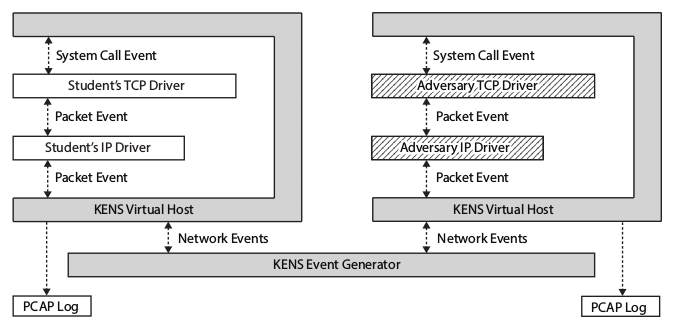
\includegraphics[width=0.85\textwidth]{04-figuras/KENVSv2.png}
    \caption{Funcionamento em camadas}
    \label{fig:KENVSv2}
    \fonte{\cite{LEE}}
\end{figure}  	 
	     % Trabalhos relacionados
% -----------------------------------------------------------------------------
% Metodologia
% -----------------------------------------------------------------------------

\chapter{Metodologia}
\label{chap:metodologia}
Com o objetivo de criar aplicações que simulem cada uma das camadas do modelo TCP/IP, foram escolhidos cinco protocolos para serem implementados. Da camada de aplicação o protocolo HTTP, utilizado para comunicação de um sistema final e um servidor Web, permitindo assim navegação pela Internet, será implementado. Da camada seguinte, a de Transporte, devido a sua importância, os dois principais protocolos serão implementados, o protocolo de transporte confiável, TCP, e o não confiável, UDP.
 
Os seguimentos recebidos da camada de transporte deverão ser tratados na camada de internet pelo protocolo IP fazendo uso do roteamento o qual, por sua vez, deverá entregar o pacote resultante para camada de Enlace. Esta terá o protocolo Ethernet simulado, complementado do protocolo ARP para tradução do endereço IP para MAC, possibilitando assim o envio do quadro para o host destino.

A Figura \ref{fig:objetivo} mostra a formulação implementada neste trabalho, representando o funcionamento da pilha de protocolos quando uma aplicação cliente, no caso o browser, faz uma requisição HTTP ao servidor. A arquitetura cliente/servidor foi utilizada para promover a interação entre as camadas, assim elas conversam entre si através de sockets, onde as portas são representadas pelo caminho aberto em cada camada e as mensagens são representadas pelas setas: vermelha ilustrando a mensagem de requisição, e azul a reposta mandada pelo servidor.


\begin{figure}[H]
	\centering
    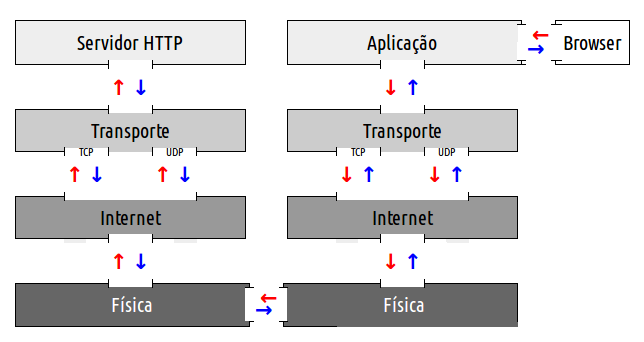
\includegraphics[width=0.80\textwidth]{04-figuras/Esquema.png}
    \caption{Esquema da arquitetura desenvolvida}
    \label{fig:objetivo}
\end{figure}

Cada camada foi implementada de forma independente, e a cada etapa os dados referentes à PDU são exibidos para, assim, manter a transparência objetivada para a utilização deste sistema como ferramente de ensino. Estes dados são estruturados de acordo com os respectivos padrões definidos pela RFC.

Objetivando a melhor forma de implementação, considerando a simplicidade e bibliotecas disponíveis para acesso baixo n\'ivel \'a rede, a linguagem escolhida foi o Python, vers\~ao 2.7. O planejamento teve como objetivo permitir a interaç\~ao entre camadas e testes a cada etapa do desenvolvimento. Desta forma o primeiro m\'odulo desenvolvido foi referente a camada F\'isica para garantir a transmiss\~ao de mensagens entre hosts. Utilizando este m\'odulo como base foram desenvolvidos, na seguinte ordem, os m\'odulos simuladores referentes \'a camada de Aplicaç\~ao, Transporte e Internet.
               % Metodologia
%% -----------------------------------------------------------------------------
% Resultados
% -----------------------------------------------------------------------------

\chapter{Análise e Discussão dos Resultados}

Cada capítulo deve conter uma pequena introdução (tipicamente, um ou dois parágrafos), em seção não numerada, que deve deixar claro o objetivo e o que será discutido no capítulo, bem como a organização do capítulo.

\section{Título da seção}
\label{sec:titSecResult}

Inserir seu texto aqui...
                % Resultados
%% -----------------------------------------------------------------------------
% Conclusão
% -----------------------------------------------------------------------------

\chapter{Conclusão}
\label{chap:conclusao}

Procure fazer uma análise crítica de seu trabalho, destacando os principais resultados e as contribuições deste trabalho para a área de pesquisa.

\section{Trabalhos Futuros}
\label{sec:trabalhosFuturos}

Também deve indicar, se possível e/ou conveniente, como este trabalho pode ser estendido ou aprimorado.

\section{Considerações Finais}
\label{sec:consideracoesFinais}

As derradeiras palavras para encerramento do seu trabalho acadêmico.

% -----------------------------------------------------------------------------
% OBS: a norma ABNT estabelece que em qualquer tipo de trabalho acadêmico monográfico
% deve haver um capítulo de conclusão
% -----------------------------------------------------------------------------
                 % Conclusão
%% -----------------------------------------------------------------------------
% Introdução
% -----------------------------------------------------------------------------

\chapter{Pré relatório}
\label{chap:pre-relatorio}



\section{Introdução}
\label{sec:antesleiame}

O impacto da internet no cotidiano do ser humano hoje, pode ser considerado imensurável, está presente em nossas vidas de várias formas e intensidades. \cite{Fourouzan} define a internet como a composição de duas ou mais redes (grupo de dispositivos conectados que se comunicam) que podem, por sua vez, comunicar entre si. Em outras palavras: a Internet é um método de interconexão de redes físicas e um conjunto de convenções para uso de redes que permite a interação dos computadores que elas alcançam \cite{Comer} (no contexto atual, podemos considerar computadores como qualquer dispositivo final que tenha capacidade de acesso à internet).

Todas as atividades na internet que envolvem duas ou mais entidades remotas comunicantes são governadas por um protocolo, o qual define um formato e a ordem das mensagens trocadas entre estas entidades, bem como as ações realizadas na transmissão e/ou no recebimento de uma mensagem ou outro evento \cite{Kurose}.

Em 1973, Cerf e Kahn, delinearam estes protocolos, considerados uma nova versão do NCP (Network Control Protocol, software que fornecia a comunicação entre hosts). O artigo publicado sobre o protocolo de controle de transmissão (TCP) incluía conceitos como encapsulamento, datagrama e funções de gateway \cite{Forouzan}. O modelo de protocolos TCP/IP é constituído de cinco camadas: física, enlace de dados, rede, transporte e aplicação. 

Posteriormente os protocolos de controle de transmissão TCP foi dividido em dois protocolos distintos: TCP (Transmission Control Protocol) e IP (Internetworking Protocol). O IP traria o roteamento de datagramas enquanto o TCP seria responsável pelas funções de níveis mais altos, como segmentação, remontagem e detecção de erros. O protocolo de interligação em rede tornou-se então conhecido como TCP/IP \cite{Forouzan}.

Em 1983, o TCP/IP tornou-se o protocolo oficial (em detrimento dos protocolos originais da ARPANET). Ou seja, a partir de então, para usar a Internet para acessar um computador em uma rede diferente, tornou-se necessário executar o TCP/IP. Ele é oficalmente definido pelo RFC 1180 \cite{rfc}: RFCs são documentos técnicos desenvolvidos e mantidos pelo IETF (Internet Enginnering Task Force), instituição que especifica os padrões que serão implementados e utilizados em toda a internet.

Hoje em dia temos \'a nossa disposi\c{c}\~ao alguns softwares com o objetivo de simular o funcionamento completo de uma rede, como exemplo o Cisco Packege Tracer \cite{CiscoPT} e o GNS3 \cite{GNS3}. Ambos s\~ao softwares dispon\'iveis gratuitamente e direciocionados para principalmente para o meio acad\^emico. O Cisco Packege Tracer \cite{CiscoPT} vai além e permite simular protocolos e visualizá-los. No trabalho de conclusão de curso Poletti \cite{Poletti} utilizou como base um simulador e implementou novas funcionalidades e aperfeiçoamento de recursos enfatizando as etapas que ocorrem no estabelecimento de conexão TCP.


\section{Motivação e objetivo}
\label{sec:justificativa}

Dada tal importância ao modelo TCP/IP é de grande relevância o entendimento deste e seu funcionamento em cursos voltados para área de tecnologia que tem a disciplina de rede em seu currículo, como Engenharia da Computação, Engenharia Elétrica, Sistemas de Informação e etc. Com o objetivo de facilitar o aprendizado e o conhecimento de como este modelo se comporta foi idealizado neste trabalho a construção de aplicações que simulem cada camada presentes no modelo TCP/IP separadamente, permitindo que essa comunicação flua em uma rede normal.

\section{Relevância}
\label{sec:motivacao}

A contribuição pretendida por esta proposta encontra-se no contexto educacional: criar uma ferramenta de ensino capaz de aprofundar o aprendizado dando uma visão mais aprofundada sobre a pilha de protocolos do modelo TCP/IP.

\section{Metodologia}
\label{metodologia}

\begin{enumerate}
	\item Revisar literatura e pesquisa de artigos publicados que contemplem a área.
	\item Contemplar possíveis soluções para o problema e avaliar linguagens de programação mais adequada para a implementação.
	\item Planejar a arquitetura do software e desenvolvimento.
	\item Realizar sistemática de testes comparando resultados obtidos e desejados.
	\item Analisar os resultados, elaborar a conclusão e documentação.
\end{enumerate}

\section{Infraestrutura necessária}
\label{infra}

Para o desenvolvimento deste trabalho será necessário dois computadores, com sistema operacional Linux, conectados em uma mesma rede.

\section{Resultados esperados}
\label{sec:organizacaoTrabalho}

Este trabalho deve desenvolver quatro aplicações distintas, que representem as camadas de aplicação, transporte, rede e enlace de dados. A comunicação ponto a ponto deverá ocorrer por meio do modelo cliente servidor sobre uma rede existente.

A proposta \'e que haja um monitoramento do funcionamento em camadas a apartir de uma implementa\c{c}\~ao (a ser definida no projeto) para a valida\c{c}\~ao das PDU's que foram trocadas entre camadas.



\section{Cronograma}
\label{cronos}

\begin{table}[H]
\centering
%\caption{My caption}
\label{my-label}
\resizebox{\textwidth}{!}{
\begin{tabular}{l|l|l|l|l|l|l|l|l|l|}
\cline{2-10}
                                                                & Março                                           & Abril                    & Maio                     & Junho                    & Julho                    & Agosto                   & Setembro                 & Outubro                  & Novembro                 \\ \hline
\multicolumn{1}{|l|}{Definição do Tema}                         & \cellcolor{black} &                          &                          &                          &                          &                          &                          &                          &                          \\ \hline
\multicolumn{1}{|l|}{Elaboração e entrega do pré projeto}       & \cellcolor{black}                        &                          &                          &                          &                          &                          &                          &                          &                          \\ \hline
\multicolumn{1}{|l|}{Revisão de Literatura}                     & \cellcolor{black}                        & \cellcolor{black} &                          &                          &                          &                          &                          &                          &                          \\ \hline
\multicolumn{1}{|l|}{Avaliar possíveis soluções para o projeto} &                                                 & \cellcolor{black} & \cellcolor{black} &                          &                          &                          &                          &                          &                          \\ \hline
\multicolumn{1}{|l|}{Planejamento da arquitetura do software}   &                                                 &                          & \cellcolor{black} &                          &                          &                          &                          &                          &                          \\ \hline
\multicolumn{1}{|l|}{Elaboração e entrega do TCC1}              &                                                 &                          & \cellcolor{black} & \cellcolor{black} &                          &                          &                          &                          &                          \\ \hline
\multicolumn{1}{|l|}{Desenvolvimento}                           &                                                 &                          &                          &                          & \cellcolor{black} & \cellcolor{black} & \cellcolor{black} &                          &                          \\ \hline
\multicolumn{1}{|l|}{Testes}                                    &                                                 &                          &                          &                          &                          &                          & \cellcolor{black} &                          &                          \\ \hline
\multicolumn{1}{|l|}{Análise dos resultados}                    &                                                 &                          &                          &                          &                          &                          &                          & \cellcolor{black} &                          \\ \hline
\multicolumn{1}{|l|}{Elaboração e entrega do TCC2}              &                                                 &                          &                          &                          &                          &                          &                          & \cellcolor{black} & \cellcolor{black} \\ \hline
\end{tabular}}
\end{table}






% Insere os elementos pós-textuais
\postextual
% -----------------------------------------------------------------------------
% Referências
% -----------------------------------------------------------------------------

% -----------------------------------------------------------------------------
% Carrega o arquivo "base-referencias.bib" e extrai automaticamente as referências citadas
% -----------------------------------------------------------------------------

\bibliography{./base-referencias}{}
\bibliographystyle{abntex2-alf} % Define o estilo ABNT para formatar a lista de referências

% -----------------------------------------------------------------------------
% Este arquivo não necessita de ser editado.
% -----------------------------------------------------------------------------
           % Referências
%% -----------------------------------------------------------------------------
% Apêndices
% -----------------------------------------------------------------------------

\begin{apendicesenv}
\partapendices

% -----------------------------------------------------------------------------
% Primeiro apêndice
% -----------------------------------------------------------------------------

\chapter{Nome do apêndice} % Edite para alterar o título deste apêndice
\label{chap:apendiceA}

Lembre-se que a diferença entre apêndice e anexo diz respeito à autoria do texto e/ou material ali colocado.

Caso o material ou texto suplementar ou complementar seja de sua autoria, então ele deverá ser colocado como um apêndice. Porém, caso a autoria seja de terceiros, então o material ou texto deverá ser colocado como anexo.

Caso seja conveniente, podem ser criados outros apêndices para o seu trabalho acadêmico. Basta recortar e colar este trecho neste mesmo documento. Lembre-se de alterar o "label"{} do apêndice.

Não queira colocar tudo que é complementar em um único apêndice. Organize seus apêndices de modo a que, em cada um deles, haja um único tipo de conteúdo. Isso facilita a leitura e compreensão para o leitor do trabalho. É para ele que você escreve.

% -----------------------------------------------------------------------------
% Novo apêndice
% -----------------------------------------------------------------------------

\chapter{Estrutura de trabalhos acadêmicos}
\label{chap:apEstrTrabAcad}

Quanto à estrutura do trabalho acadêmico, esta varia sobremaneira, a depender da conveniência do autor e seu(s) respectivo(s) orientador(es). No entanto, de acordo com as normas ABNT, alguns elementos são obrigatórios.

A título de sugestão, e apenas isso, a \autoref{fig:estrutura-projeto-qualificacao} apresenta uma estrutura para um projeto de qualificação de mestrado ou doutorado, conforme a norma \citeonline{NBR14724:2011}.

\begin{figure}[!htb]
    \centering
    \caption{Estrutura sugerida de um Projeto de Qualificação para os cursos de Mestrado ou Doutorado}
    \includegraphics[width=0.5\textwidth]{./04-figuras/estrutura-projeto-qualificacao}
    \label{fig:estrutura-projeto-qualificacao}
\end{figure}

Já a \autoref{fig:estrutura-tese-dissertacao} apresenta uma estrutura para uma tese de doutorado ou dissertação de mestrado, conforme a norma \citeonline{NBR14724:2011}.

Cabe ressaltar que, em todas as figuras, os elementos obrigatórios estão destacados em vermelho, os demais são opcionais.

\begin{figure}[!htb]
    \centering
    \caption{Estrutura sugerida de uma Tese de Doutorado ou Dissertação de Mestrado}
    \includegraphics[width=0.5\textwidth]{./04-figuras/estrutura-tese-dissertacao}
    \label{fig:estrutura-tese-dissertacao}
\end{figure}

Observe que a estrutura de um projeto de qualificação é muito similar à da tese ou dissertação. A única diferença existente é que num projeto de qualificação o autor certamente terá, via de regra, apenas resultados parciais e preliminares. Além disso, estando o trabalho ainda em andamento, há que se apresentar um cronograma de trabalho que evidencie que o mesmo poderá ser concluído dentro dos prazos estabelecidos pelo programa.

Por fim, como foi dito, este  \emph{template} pode ser utilizado para outros trabalhos acadêmicos. Neste caso, a \autoref{fig:estrutura-projeto-pesquisa} apresenta uma sugestão de projeto de pesquisa a ser submetido ao programa para fins de admissão ao mesmo, conforme a norma \citeonline{NBR15287:2005}.

\begin{figure}[!htb]
    \centering
    \caption{Estrutura sugerida de um projeto de pesquisa para admissão ao PPGMMC}
    \includegraphics[width=0.6\textwidth]{./04-figuras/estrutura-projeto-pesquisa}
    \label{fig:estrutura-projeto-pesquisa}
\end{figure}

Você deverá editar o arquivo principal {\ttfamily meuTrabalhoAcademico.tex} para fazer os ajustes necessários, reiterando que as estruturas apresentadas são mera sugestão.

A inclusão de reticências (\ldots) no texto deverá ser feita através de um comando especial denominado \verb|\ldots| \cite{LaTeX2014}. Assim esse comando deverá ser utilizado ao invés da digitação de três pontos.

Para melhor entendimento do uso do estilo de formatação, aconselha-se que o potencial usuário analise os comandos existentes no arquivo {\ttfamily main.tex} e os resultados obtidos no arquivo {\ttfamily main.pdf} depois do processamento pelo software \LaTeX{} + \textsc{Bib}\TeX{} \cite{LaTeX2014,BibTeX2014}.
Recomenda-se a consulta ao material de referência do software para a sua correta utilização \cite{Lamport1986,Buerger1989,Kopka2003,Mittelbach2004}.

Finalmente, este modelo apresenta um arquivo {\ttfamily makefile} para agilizar a compilação do documento \LaTeX{} e do \textsc{Bib}\TeX{}. portanto, para gerar o documento final no formato PDF, basta apenas executar o comando {\ttfamily make all} no linux. Para limpar os arquivos temporários, basta digitar o comando {\ttfamily make clean}.

O estilo de documento utilizado é o {\ttfamily abntex2}.
Através desse estilo a constituição do documento torna-se facilitada, uma vez que o mesmo possui comandos especiais para auxiliar a distribuição/definição das diversas partes constituintes do projeto.
Esse estilo é baseado nas normas da ABNT\index{ABNT}.

Maiores detalhes relacionados aos comandos existentes no estilo poderão ser adquiridos através da documentação disponível no site \href{https://code.google.com/p/abntex2/}{https://code.google.com/p/abntex2/} \cite{abnTeX22014b}.

Uma das principais vantagens do uso do estilo de formatação para \LaTeX{}  é a formatação \textit{automática} dos elementos que compõem um documento acadêmico, tais como capa, folha de rosto, dedicatória, agradecimentos, epígrafe, resumo, abstract, listas de figuras, tabelas, siglas e símbolos, sumário, capítulos, referências, etc.

% -----------------------------------------------------------------------------
% Novo apêndice
% -----------------------------------------------------------------------------

\chapter{Sobre as ilustrações}
\label{chap:apSobreIlust}

A seguir ilustra-se a forma de incluir ilustrações no corpo do texto. Pela norma figuras, tabelas, quadros, equações, quadros, algoritmos, diagrama, etc. são tipos específicos de ilustrações. As ilustrações (pelo menos alguns tipos específicos) serão indexadas automática em suas respectivas listas.

A numeração sequencial de figuras, tabelas e equações ocorre de modo automático.

Referências cruzadas são obtidas através dos comandos \verb|\label{}| e \verb|\ref{}|. Por exemplo, não é necessário saber que o número de certo capítulo é \ref{chap:fundamentacaoTeorica} para colocar o seu número no texto. Alternativamente se pode usar desta forma: \autoref{chap:fundamentacaoTeorica}. Isto facilita muito a inserção, remoção ou relocação de elementos numerados no texto (fato corriqueiro na escrita e correção de um documento acadêmico) sem a necessidade de renumerá-los todos.

\section{Figuras}
\label{sec:figuras}

Abaixo é apresentado um exemplo de figura.

A \autoref{fig:kdtree} aparece automaticamente na lista de figuras.

Para uso avançado de imagens no \LaTeX{}, recomenda-se a consulta de literatura especializada \cite{Goossens2007}.

\begin{figure}[!htb]
    \centering
    \caption{Exemplo da estrutura de uma árvore KD}
    \includegraphics[width=0.5\textwidth]{./04-figuras/figura-exemplo}
    \fonte{\citeonline{Souza2012}}
    \label{fig:kdtree}
\end{figure}

\section{Quadros e tabelas}
\label{sec:tabelas}

Também é apresentado o exemplo do \autoref{qua:comparabd} e da \autoref{tab:testes}, que aparece automaticamente na lista de quadros e tabelas.

Informações sobre a construção de tabelas no \LaTeX{} podem ser encontradas na literatura especializada \cite{Lamport1986,Buerger1989,Kopka2003,Mittelbach2004}.

\begin{quadro}[!htb]
    \centering
    \caption{Hierarquia de restrições das questões.\label{qua:comparabd}}
    \begin{tabular}{|p{7cm}|p{7cm}|}
        \hline
        \textbf{BD Relacionais} & \textbf{BD Orientados a Objetos} \\
        \hline
        Os dados são passivos, ou seja, certas operações limitadas podem ser automaticamente acionadas quando os dados são usados. Os dados são ativos, ou seja, as solicitações fazem com que os objetos executem seus métodos. & Os processos que usam dados mudam constantemente. \\
        \hline
    \end{tabular}
    \fonte{\citeonline{Carvalho2001}}
\end{quadro}


Muitos confundem, mas existem diferenças entre tabelas e quadros.

Um quadro é formado por linhas horizontais e verticais, sendo, portanto ``fechado''. Você deverá utilizar um quadro quando o conteúdo é majoritariamente não-numérico. O número do quadro e o título vem acima do quadro, e a fonte, deve vir abaixo.

Uma tabela é formada apenas por linhas verticais, sendo, portanto ``aberta''. Você deverá utilizar uma tabela quando o conteúdo é majoritariamente numérico. O número da tabela e o título vem acima da tabela, e a fonte, deve vir abaixo, tal como no quadro.

Exemplo de tabela:

\begin{table}[!htb]
    \centering
    \caption[Resultado dos testes]{Resultado dos testes.
    \label{tab:testes}}
    \begin{tabular}{rrrrr}
        \toprule
            & Valores 1 & Valores 2 & Valores 3 & Valores 4 \\
        \midrule
            Caso 1 & 0,86 & 0,77 & 0,81 & 163 \\
            Caso 2 & 0,19 & 0,74 & 0,25 & 180 \\
            Caso 3 & 1,00 & 1,00 & 1,00 & 170 \\
        \bottomrule
    \end{tabular}
\end{table}


\section{Equações}
\label{sec:equacoes}

A transformada de Laplace é dada na \autoref{eq:laplace}, enquanto a Eq. \ref{eq:dft} apresenta a formulação da transformada discreta de Fourier bidimensional\footnote{Deve-se reparar na formatação esteticamente perfeita destas equações.}. Observe que utilizamos propositalmente duas formas distintas para referenciar as equações.

\begin{equation}
    X(s) = \int\limits_{t = -\infty}^{\infty} x(t) \, \text{e}^{-st} \, dt
    \label{eq:laplace}
\end{equation}

\begin{equation}
    F(u, v) = \sum_{m = 0}^{M - 1} \sum_{n = 0}^{N - 1} f(m, n) \exp \left[ -j 2 \pi \left( \frac{u m}{M} + \frac{v n}{N} \right) \right]
    \label{eq:dft}
\end{equation}

\section{Algoritmos}\label{sec:algoritmos}

Os algoritmos devem ser feitos segundo o modelo abaixo. Para isso, utilizar o pacote {\ttfamily algorithm2e} no início do arquivo principal como neste exemplo.
\\
\\

\begin{algorithm}
    \caption{Algoritmo para remoção aleatória de vértices}
    \KwIn{o número $n$ de vértices a remover, grafo original $G(V, E)$}
    \KwOut{grafo reduzido $G'(V,E)$}
    $removidos \leftarrow 0$ \\
    \While {removidos $<$ n } {
        $v \leftarrow$ Random$(1, ..., k) \in V$ \\
            \For {$u \in adjacentes(v)$} {
                remove aresta (u, v)\\
                $removidos \leftarrow removidos + 1$\\
            }
            \If {há  componentes desconectados} {
                remove os componentes desconectados\\
            }
        }
\end{algorithm}


% -----------------------------------------------------------------------------
% Novo apêndice
% -----------------------------------------------------------------------------

\chapter{Sobre as listas}
\label{chap:apSobreLista}

Para construir listas de "\textit{bullets}"{} ou listas enumeradas, inclusive listas aninhadas, é utilizado o pacote \verb|paralist|.

O exemplo a seguir ilustra duas listas não numeradas aninhadas, utilizando o ambiente \verb|\itemize|. Observe a indentação, bem como a mudança automática do tipo de "\textit{bullet}"{} nas listas aninhadas.

\begin{itemize}
    \item item não numerado 1
    \item item não numerado 2
    \begin{itemize}
        \item subitem não numerado 1
        \item subitem não numerado 2
        \item subitem não numerado 3
    \end{itemize}
    \item item não numerado 3
\end{itemize}

Por outro lado, o exemplo a seguir ilustra duas listas numeradas aninhadas, utilizando o ambiente \verb|\enumerate|. Observe a numeração progressiva e indentação das listas aninhadas.

\begin{enumerate}
    \item item numerado 1
    \item item numerado 2
    \begin{enumerate}
        \item subitem numerado 1
        \item subitem numerado 2
        \item subitem numerado 3
    \end{enumerate}
    \item item numerado 3
\end{enumerate}

Cabe ressaltar que os ambientes \verb|\itemize| e \verb|\enumerate| podem ser utilizados alternativamente. No entanto, durante a compilação pdflatex são apresentados erros associados a estes ambientes, porém o pdf é gerado corretamente. Trata-se de um "\textit{bug}"{} que ainda não conseguimos resolver. Caso conheça a solução, por favor, comunique-nos para que possamos incluí-la numa futura atualização deste modelo.

% -----------------------------------------------------------------------------
% Novo apêndice
% -----------------------------------------------------------------------------

\chapter{Sobre citações e chamadas de referências}
\label{chap:apSobreCita}

Citações são trechos transcritos ou informações retiradas das publicações consultadas para a realização do trabalho.
As citações são utilizadas no texto com o propósito de esclarecer, completar, embasar ou corroborar as ideias do autor.

Todas as publicações consultadas e efetivamente utilizadas (por meio de citações) devem ser listadas, obrigatoriamente, nas referências bibliográficas, de forma a preservar os direitos autorais e intelectuais.

A norma ABNT NBR:10520-2002 classifica as citações em: citações livres e citações literais.

\section{Citações livres}
\label{sec:citacoesLivres}

Nas citações livres, reproduzem-se as ideias e informações de um autor, sem, entretanto, ``copiar letra por letra'' o texto do autor. Sendo assim, não há muito a dizer sobre como fazer citações livres, exceto que há que se tomar o devido cuidado com o "recortar e colar e modificar"{} para que não se caracterize plágio.

Quanto à chamada da referência, ela pode ser feita de duas maneiras distintas, conforme o nome do(s) autor(es) façam parte do seu texto ou não. Os exemplos a seguir ilustram estas duas possibilidades.

Enquanto \citeonline{Maturana2003} defendem uma epistemologia baseada na biologia. Para os autores, é necessário rever \ldots.

Por outro lado, \citeonline{Barbosa2004} contra-argumenta afirmando que \ldots.

Acima, as chamadas de referências foram feitas com o comando \verb|\citeonline{chave}|, que produzirá a formatação correta, conforme a norma ABNT.

Observe que em ambos os casos anteriores, a frase fica incompleta e incompreensível caso as palavras "Maturana e Varela"{} e "Barbosa et al."{} não sejam "pronunciadas"{}. Ou seja, os nomes dos autores fazem parte da frase. Neste caso, a formatação automática da chamada de referência coloca os nomes dos autores seguido, entre parêntesis pelo ano de publicação da obra referenciada. Isso apenas no caso em que se usa o esquema autor-ano, que é \textit{padrão} neste modelo \LaTeX{}.

A segunda maneira de fazer uma chamada de referência deve ser utilizada quando se quer evitar uma interrupção na sequência do texto, o que poderia, eventualmente, prejudicar a leitura.

Assim, a citação livre é feita e imediatamente após a obra referenciada deve ser colocada entre parênteses. Porém, neste caso específico, o nome do autor deve vir em caixa alta, seguido do ano da publicação, como nos exemplos a seguir.

Há defensores da epistemologia baseada na biologia que argumentam em favor da necessidade de \ldots \cite{Maturana2003}.

Por outro lado, há os que contra-argumentam afirmando que \ldots  \cite{Barbosa2004}.

Nos dois casos imediatamente acima a chamada de referência deve ser feita com o comando \verb|\cite{chave}|, que produzirá a formatação correta, conforme a norma ABNT.

Observe que o estilo de redação das frases teve que ser modificado para torná-las compreensíveis sem a menção explícita dos nomes dos autores. Estes agora não são parte integrante da frase, ficam entre parêntesis. Neste caso, a formatação automática da chamada de referência coloca, entre parêntesis, os nomes dos autores seguido pelo ano de publicação da obra referenciada. Novamente, apenas no caso em que se usa o esquema autor-ano, que é \textit{padrão} neste modelo \LaTeX{}.

Por fim, cabe chamar a atenção para o detalhe do termo \textit{et al.} que deve ser utilizado quando o trabalho citado possui mais de três autores. Esse recurso é automatizado pelo estilo {\ttfamily abntex2}. Caso não haja desejo em abreviar o nome dos demais autores através do termo \textit{et al.}, deve-se incluir a opção {\ttfamily abnt-no-etal-label}.

\section{Citações literais}
\label{sec:citacoesLiterais}

Nas citações literais, reproduzem-se as ideias e informações de um autor, exatamente como este a expressou, ou seja, faz-se uma ``cópia letra por letra'' do texto do autor. Sendo assim, obviamente, a obra citada deve ser referenciada, sob pena de se caracterizar plágio.

Quanto à chamada da referência, ela pode ser feita de qualquer das duas maneiras mencionadas na \autoref{sec:citacoesLivres}, conforme o nome do(s) autor(es) façam parte do seu texto ou não.

Há duas maneiras distintas de se fazer uma citação literal, conforme o trecho citado seja longo ou curto.

Quando o trecho citado é longo (4 ou mais linhas) deve-se usar um parágrafo específico para a citação, na forma de um texto recuado (4 cm da margem esquerda), com tamanho de letra menor do aquela utilizada no texto e espaçamento entrelinhas simples. Veja o exemplo abaixo.

\begin{citacao}
    Desse modo, opera-se uma ruptura decisiva entre a reflexividade filosófica, isto é a possibilidade do sujeito de pensar e de refletir, e a objetividade científica.     Encontramo-nos num ponto em que o conhecimento científico está sem consciência. Sem consciência moral, sem consciência reflexiva e também subjetiva. Cada vez mais o desenvolvimento extraordinário do conhecimento científico vai tornar menos praticável a própria possibilidade de reflexão do sujeito sobre a sua pesquisa \cite[p.~28]{Silva2000}.
\end{citacao}

Para se criar o efeito demonstrado na citação anterior, deve-se utilizar o comando:

\begin{verbatim}
\begin{citacao}
<citacao>
\end{citacao}
\end{verbatim}

Acima, para a chamada da referência o comando \verb|\cite[p.~28]{Silva2000}| foi utilizado, visto que os nomes dos autores não são parte do trecho citado.

Observe ainda que foi indicado o número da página da obra citada que contém o trecho citado. A localização precisa do trecho citado deve ser indicada sempre, exceto para artigos científicos (tipicamente com poucas páginas, o que geralmente não é o caso de artigos de revisão de literatura) e outros documentos com "poucas"{} páginas.

Alternativamente, é possível construir uma frase que contenha os autores, e irá encaminhar (por assim dizer) a citação literal. Assim sendo, note que pode após a citação literal não mais aparece o nome dos autores, visto que já se encontra no texto. Veja o exemplo seguinte.

No entanto, \citeonline[p.~33]{Silva2000}, ao fazerem as suas críticas à ciência moderna, afirmam:

\begin{citacao}
    Mas o curioso é que o conhecimento científico que descobriu os meios realmente extraordinários para, por exemplo, ver aquilo que se passa no nosso sol, para tentar conceber a estrutura das estrelas extremamente distantes, e até mesmo para tentar pesar o universo, o que é algo de extrema utilidade, o conhecimento científico que multiplicou seus meios de observação e de concepção do universo, dos objetos, está completamente cego, se quiser considerar-se apenas a si próprio!
\end{citacao}

Já quando o trecho citado é curto (3 ou menos linhas) ele deve inserido diretamente no texto entre aspas. Veja os dois exemplos seguintes, cada qual utilizando uma forma de chamada de referência.

A epistemologia baseada na biologia parte do princípio de que ``assumo que não posso fazer referência a entidades independentes de mim para construir meu explicar'' \cite[p.~35]{Maturana2003}.

A epistemologia baseada na biologia de \citeonline[p.~35]{Maturana2003} parte do princípio de que ``assumo que não posso fazer referência a entidades independentes de mim para construir meu explicar''.

Finalmente, e isto vale para citações curtas ou longas, caso seja necessário inserir ou suprimir (modificar de modo geral) qualquer palavra ou frase no trecho citado literalmente, qualquer que seja a finalidade, isto deve ser feito colocando sua intervenção entre colchetes retos e deve ser indicado explicitamente ao final da citação. Veja o exemplo seguinte.

A epistemologia baseada na biologia parte do princípio de que ``assumo que não posso fazer referencia [\textit{sic}] a \underline{entidades independentes} de mim [realidade objetiva] para construir meu explicar'' \cite[p.~35, comentários e grifo nosso]{Maturana2003}.

\section{Mais detalhes sobre as chamadas de referências}
\label{sec:referUtilizadas}

A seguir há mais exemplos dos comandos para as chamadas de referências e o resultado produzido.

\citeonline{Maturana2003} \ \ \  \verb|\citeonline{Maturana2003}|\\
\citeonline{Barbosa2004} \ \ \   \verb|\citeonline{Barbosa2004}|\\
\cite[p.~28]{Silva2000} \ \ \  \verb|\cite[p.~28]{Silva2000}|\\
\citeonline[p.~33]{Silva2000} \ \ \   \verb|\citeonline[p.~33]{v}|\\
\cite[p.~35]{Maturana2003} \ \ \   \verb|\cite[p.~35]{Maturana2003}|\\
\citeonline[p.~35]{Maturana2003} \ \ \   \verb|\citeonline[p.~35]{Maturana2003}|\\
\cite{Barbosa2004,Maturana2003} \ \ \   \verb|\cite{Barbosa2004,Maturana2003}|\\

Há que se tomar bastante cuidado com referências cujos autores têm nomes compostos, tipo João de Souza Júnior ou Antônio José da Silva Filho. Para que a formatação seja correta, os nomes dos autores no arquivo {\ttfamily .bib} deverá ser cadastrado de uma forma específica. Para maiores detalhes, veja o \autopageref{chap:anexoB} \footnote{O texto do anexo é de inteira responsabilidade do autor devidamente referenciado.}.

Os exemplos abaixo ilustram a formatação correta.

\cite[p.~28]{vanGELDER1998} \ \ \ \ \  \verb|\cite[p.~28]{vanGELDER1998}|\\
\citeonline[p.~28]{vanGELDER1998} \ \ \ \ \  \verb|\citeonline[p.~28]{vanGELDER1998}|\\

Observe que, a despeito do que está dito no \autoref{chap:anexoB}, ainda há falhas na formatação ABNT de nomes tipo \verb|van Gelder| quando utilizados em chamadas de referências que fazem parte do texto (\textit{e.g.}, \verb|\citeonline{vanGELDER1998}| que deveria produzir \verb|van Gelder (1998)|). Este problema pode ser contornado facilmente, simplesmente evitando o uso dessa forma de chamada de referência, preferindo sempre nestes casos, o uso da forma \textit{e.g.}, \verb|\cite{vanGELDER1998}| que será formatada corretamente, produzindo \verb|(van GELDER, 1998)|.

Observe ainda o caso em que é feita duas citações juntas \cite{Santos2003, Neubert2001} e como citar endereços Web \cite{IRL2014}.

% -----------------------------------------------------------------------------
% Novo apêndice
% -----------------------------------------------------------------------------

\chapter{Sobre as referências bibliográficas}
\label{chap:apSobreRefer}

A bibliografia é feita no padrão \textsc{Bib}\TeX{}. As referências são colocadas em um arquivo separado. Os elementos de cada item bibliográfico que devem constar nas referências bibliográficas são apresentados a seguir. Tais referências bibliográficas devem seguir a norma \citeonline{NBR6023:2002} da ABNT\footnote{As normas técnicas da ABNT não são gratuitas.}.

\section{Entradas de referências}
\label{sec:entradasRefs}

Entradas são objetos de citação bibliográficas. Dito de outra forma, são as categorias dos tipos de documentos e materiais componentes da bibliografia. A classe abn\TeX{} define as seguintes entradas:

\begin{verbatim}
@book
@inbook
@article
@phdthesis
@mastersthesis
@monography
@techreport
@manual
@proceedings
@inproceedings
@journalpart
@booklet
@patent
@unpublished
@misc
\end{verbatim}

Cada entrada é formatada pelo pacote \citeonline{abnTeX22014d} de uma forma específica. Algumas entradas foram introduzidas especificamente para atender à norma \citeonline{NBR6023:2002}, são elas: \verb|@monography|, \verb|@journalpart|,\verb|@patent|. As demais entradas são padrão \textsc{Bib}\TeX{}. Para maiores detalhes, refira-se a \citeonline{abnTeX22014d}, \citeonline{abnTeX22014b}, \citeonline{abnTeX22014c}.

A entrada \verb|@monography| é utilizada para cadastrar referências a trabalhos de conclusão de curso, monografias de cursos de especialização (pós-graduação \textit{lato sensu}), e outros trabalhos monográficos, exceto dissertação de mestrado e tese de doutorado. Eu particularmente, não considero que a formatação deste tipo de entrada está adequado. Para um trabalho de conclusão de curso (TCC) de curso de graduação, que deveria ser formatado como "[\ldots] Trabalho de Conclusão de Curso (Bacharelado em Engenharia de Computação) [\ldots]"{}; no entanto o uso de \verb|@monography| irá produzir "[\ldots] Monografia (Bacharelado em Engenharia de Computação) [\ldots]"{}. A própria  \citeonline{NBR6023:2002}, na seção 8.11.4, apresenta um exemplo com a formatação diferente daquela proporcionada por \citeonline{abnTeX22014d}.

A entrada \verb|@journalpart| é utilizada, conforme diz o manual \cite{abnTeX22014d}, para cadastrar referências e formatar partes de periódicos. Não fica claro o que se quer dizer com partes de journal. Em alguns casos, tais partes são artigos - e portanto, deveriam ser registradas como \verb|@article| - noutros casos, parece serem matérias ou textos em revistas ou jornais (não científicos). Salvo melhor juízo, me parece que esta entrada deve ser utilizada apenas neste último contexto.

A entrada \verb|@patent| é utilizada, obviamente, para cadastrar referências a patentes.

Todavia, o fato é que a normalização de referências conforme a norma \citeonline{NBR6023:2002} requer que muitos dos campos do \textsc{Bib}\TeX{} sejam adaptados. Sendo mais explícito, ao baixar um arquivo {\ttfamily .bib} de um trabalho, principalmente ser for internacional, e inserí-lo "\textit{as is}"{} em suas referências, há grande chance dessa referência ser formatada de modo errado, no que concerne à norma \citeonline{NBR6023:2002}. Isso é especialmente válido em alguns tipos de documentos de largo uso no meio acadêmico afim às áreas de Ciências Exatas, da Terra e Engenharias.

Diante disso, para evitar erros de formatação, o correto é após baixar o arquivo {\ttfamily .bib} de um trabalho, editá-lo com um editor ASCII (usando codificação UTF8), para verificar se os campos descritores que o \textit{publishers} original utilizou são aqueles requeridos pela norma ABNT.

Neste contexto, e para esta finalidade, nas seções seguintes é apresentado uma série de exemplos, quase todos, utilizados como exemplos na própria norma \citeonline{NBR6023:2002}. Para detalhes dos campos utilizados confira o arquivo {\ttfamily myRefs.bib}. Deve-se estar atento para o fato de que o uso de um sistema de gerenciamento de referências para abrir e/ou editar o arquivo {\ttfamily myRefs.bib}, pode ocultar campos utilizados pela norma ABNT e, por outro lado, exibir campos não utilizados por ela. Ou seja, o aplicativo deve ser configurado adequadamente para exibir \textbf{todos os campos}, mesmo os opcionais.

\section{Notas de rodapé}
\label{sec:notasRodape}

A norma \citeonline{NBR10520:2002}, em sua seção \textbf{7 Notas de rodapé}, classifica as notas de rodapé em duas categorias: notas explicativas\footnote{é o tipo mais comum de notas que destacam, explicam e/ou complementam o que foi dito no corpo do texto, como esta nota de rodapé, por exemplo.} e notas de referências. Já as notas de referências, como o próprio nome ja indica, são utilizadas para colocar referências e/ou chamadas de referências sob certas condições.

\subsection{Notas de referências: uso de idem, ibidem, opus citatus e outros}
\label{subsec:notasRefs}

Como indica o próprio nome, as notas de referências se prestam como recurso auxiliar para referenciação de bibliografia, e seu uso e aplicação são descritos na seção \textbf{7.1 Notas de referência} da norma \citeonline{NBR10520:2002}.

Estes recursos se referem ao uso de certas expressões consagradas para facilitar a elaboração de referencias. São eles:

\begin{itemize}
    \item idem = mesmo autor,
    \item ibidem = mesma obra,
    \item opus citatum = obra citada,
    \item locus citatum = no lugar citado,
    \item passim = aqui e alí,
    \item cf = confira,
    \item et sequentia = e sequência.
\end{itemize}

Observe que estes recursos não se adequam para serem utilizados em listas de referências bibliográficas, nem tampouco no corpo do texto. Assim, devem ser utilizados apenas nas notas de referência posicionadas no rodapé \cite[p.~6]{abnTeX22014c}, quando se referem a uma referência já feita anteriormente no corpo do texto. Ademais, essas expressões fazem sentido apenas quando aplicadas a citações de uma única referência por vez. Enfim, trata-se mais de um recurso estilístico do que algo de primeira necessidade, pelo menos para o tipo de documento usualmente elaborados nas área de Ciências Exatas, da Terra e Engenharias.

Veja o uso desses tipos de expressões nos exemplos seguintes:

\Idem[p.~21]{abnTeX22014d}

\Ibidem[p.~7]{abnTeX22014c}

\opcit[p.~9]{abnTeX22014c}

\passim{abnTeX22014c}

\cfcite[p.~3]{abnTeX22014b}

\etseq[p.~6]{abnTeX22014c}

\section{Datas em referências}
\label{sec:datasBib}

Quando as chamadas de referências são feitas no modelo autor-ano, como é o caso deste modelo \LaTeX{}, é evidente que o autor e sobretudo o ano adquirem papel de destaque. No caso da data de publicação, esta deve sempre estar presente (é elemento essencial) e indicada em algarismos arábicos.

A norma ABNT não permite o uso de expressões do tipo "sem data"{} ("[s.d]") para indicar que não se sabe a data de publicação de certa referência bibliográfica. Assim sendo, quando a data não puder ser indicada precisamente, deve-se registrar uma data aproximada entre colchetes, conforme descrito a seguir:

[1971 ou 1972] \ \ \ \ \ um ano ou outro,

[1969?] \ \ \ \ \ ano provável,

[1973] \ \ \ \ \ ano certo, não indicada no item,

[entre 1906 e 1912] \ \ \ \ \ use intervalos menores de 20 anos,

[ca. 1960] \ \ \ \ \ \textit{circa} de ... ( data aproximada),

[197-] \ \ \ \ \ década certa,

[197-?] \ \ \ \ \ década provável,

[18--] \ \ \ \ \ século certo,

[18--?] \ \ \ \ \ século provável.

\end{apendicesenv}
             % Apêndices
%% -----------------------------------------------------------------------------
% Anexos
% -----------------------------------------------------------------------------

\begin{anexosenv}
\partanexos

% -----------------------------------------------------------------------------
% Primeiro anexo
% -----------------------------------------------------------------------------

\chapter{Nome do anexo}     % edite para alterar o título deste anexo
\label{chap:anexoA}

Lembre-se que a diferença entre apêndice e anexo diz respeito à autoria do texto e/ou material ali colocado.

Caso o material ou texto suplementar ou complementar seja de sua autoria, então ele deverá ser colocado como um apêndice. Porém, caso a autoria seja de terceiros, então o material ou texto deverá ser colocado como anexo.

Caso seja conveniente, podem ser criados outros anexos para o seu trabalho acadêmico. Basta recortar e colar este trecho neste mesmo documento. Lembre-se de alterar o "label"{} do anexo.

Organize seus anexos de modo a que, em cada um deles, haja um único tipo de conteúdo. Isso facilita a leitura e compreensão para o leitor do trabalho. É para ele que você escreve.

% -----------------------------------------------------------------------------
% Novo anexo
% -----------------------------------------------------------------------------

\chapter{Dica: nomes no BibTeX}
\label{chap:anexoB}

Se você utiliza LaTeX para a redação de artigos já deve ter se deparado com algum tipo de problema no modo como o nome dos autores é apresentado no documento final (pior é quando a "descoberta"{} ocorre depois de já ter submetido o paper). Muitas vezes é difícil encontrar uma maneira certa de escrever o nome no arquivo *.bib e garantir que ele seja transcrito corretamente independente do estilo utilizado. Este texto tem o intuito de discutir o modo como o BibTeX interpreta o nome dos autores e ajudar na árdua tarefa de organizar a bibliografia.

Pessoalmente eu prefiro fornecer o nome completo dos meus autores para o BibTeX, sem abreviações e sem omitir nomes, quando possível. Desse modo, eu dou garantia que a minha bibliografia irá conter todos os dados para referenciar o autor independente do estilo utilizado para apresentá-lo. Depois disso, eu simplesmente espero que o BibTeX faça a abreviação e a colocação dos nomes da maneira correta de acordo com o estilo indicado. No entanto, para que essa tarefa seja feita é preciso apresentar os nomes da maneira correta para que a sua divisão seja feita de forma apropriada.

Para entender como o BibTeX divide um nome, é preciso conhecer antes as diversas partes que podem compor o nome de uma pessoa, que, a princípio, são: primeiro nome, nome do meio, ligação, último nome e júnior. A descrição de cada uma dessas partes é feita a seguir.

\begin{itemize}
    \item \textbf{Primeiro nome:} é o nome da pessoa, geralmente utilizado para identificar uma pessoa em um contexto informal. Ex.: Diego, João, Maria etc. Em alguns casos o primeiro nome pode ser composto por dois nomes, como Maria Ana, Victor Hugo, etc. Nestes casos, deve-se observar como a pessoa utiliza o nome para poder diferenciar a segunda parte como Primeiro nome ou Nome do meio.

    \item \textbf{Nome do meio:} é o nome que sucede o primeiro nome, mas antecede o último nome, geralmente abreviado, por simplicidade. Ex.: Alan Mathison Turing, "Mathison"{} é o nome do meio. É comum uma pessoa possuir mais do que um nome do meio e também é comum que o nome do meio de alguns autores seja desconhecido, devido às abreviações e omissões feitas pelo mesmo.

    \item \textbf{Ligação:} também chamado de separador, são as palavras "de"{}, "da"{}, "do"{}, "e"{}, "von"{}, entre outras que ligam um nome ao outro. Em John von Neumann e Ricardo Luis de Azevedo da Rocha, por exemplo, as palavras "von"{}, "de"{}  e "da"{}  são as ligações. Num contexto geral, elas normalmente são grafadas com inicial minúscula para não serem confundidas com o nome do meio e, embora não seja comum em todos lugares do mundo, no Brasil é comum um nome possuir até mais do que uma ligação.

    \item \textbf{Último nome:} também chamado de nome de família, é o nome utilizado para identificar uma pessoa em situações formais, como referência em artigos, livros etc. Ex.: Albert Einstein, "Einstein"{} é o último nome.

\item \textbf{Júnior:} é um sufixo do nome que indica a existência de um parente com o mesmo nome. Geralmente abreviado como "Jr."{} pode ser apresentado de diversas formas como "Filho"{}, "Neto"{} ou traduzido para o idioma de origem do dono do nome, como "fils"{} (filho) em francês. Ex.: John Forbes Nash Jr.
\end{itemize}

Quando indicamos o nome de um autor no BibTeX ele interpreta os nomes seguindo uma das três regras a seguir:

\begin{enumerate}
    \item \textbf{Nenhuma vírgula:} {Primeiro nome} {ligação} {Último nome}

    \item \textbf{Uma vírgula:} {ligação} {Último nome}, {Primeiro nome}

    \item \textbf{Duas vírgulas:} {ligação} {Último nome}, {Júnior}, {Primeiro nome}
\end{enumerate}

Como pode-se notar, a distinção entre essas três possíveis interpretações se dá com base na quantidade de vírgulas que foram inseridas e no posicionamento da ligação, que devem sempre ser escritas com a inicial minúscula. O(s) nome(s) do meio são todos os nomes que estão após o primeiro nome, porém antes da ligação e do último nome. A princípio, o BibTeX interpreta os nomes do meio como sendo parte do primeiro nome.

Para mostrar como isso pode gerar problemas, imagine, por exemplo, se o nome "John Forbes Nash Jr."{} fosse apresentado em um arquivo BibTeX. Como nenhuma vírgula foi inserida, será entendido que "John Forbes Nash"{} é o primeiro nome e "Jr."{} é o último nome, o que não seria correto. De forma semelhante, se for apresentado na forma "Nash Jr., John Forbes", então "John Forbes"{} será o primeiro nome enquanto "Nash Jr."{} será o último nome, que também está incorreto.

Portanto, a maneira correta de referenciar seria utilizando a terceira opção pois é a única que inclui o Jr. (utilizando duas vírgulas): "Nash, Jr., John Forbes"{}, fazendo com que "John Forbes"{} seja compreendido como primeiro nome, "Nash"{} como último nome e "Jr."{} como o júnior.

Outro grande problema ocorre quando um nome possui mais do que uma ligação, como em "Ricardo Luis de Azevedo da Rocha"{}. Quando o BibTeX lê um nome como esse, ele entende que tudo que vem após o ligador, faz parte do último nome. Neste caso, "Ricardo Luis"{} seria tratado como o primeiro nome e "Azevedo da Rocha"{} como último nome.

Para evitar esse comportamento, devemos optar pela segunda opção (utilizando uma vírgula), ou seja, "da Rocha, Ricardo {Luis de} Azevedo"{}, fazendo com que o último nome seja somente "Rocha"{} e precedido pelo seu ligador.

Note que neste último exemplo o ligador e o nome que o antecede foram delimitados por chaves. Este é um pequeno e útil truque que pode ser feito para garantir que os ligadores não sejam inclusos ao abreviar nomes (Ex.: Universidade de São Paulo, abrevia-se U.S.P. ao invés de U. de S.P. ou U.d.S.P.). Fazendo isso, o BibTeX passa a tratar "Luis de"{} como um único nome e o abrevia corretamente quando necessário.

E qual a importância de garantir que o BibTeX interprete corretamente as diversas partes de um nome? A verdade é que cada estilo trata o nome de uma maneira diferente: o IEEE, por exemplo, coloca apenas as iniciais do primeiro nome e a ligação seguida do último nome; a Nature, por outro lado, coloca a ligação e o último nome, seguido das iniciais do primeiro nome; e assim por diante. Assim sendo, entender como os nomes são interpretados nos ajuda a garantir que o mesmo seja sempre dividido da maneira correta e formatado apropriadamente independente do estilo fornecido.

Por fim, e não menos importante, também deixo aqui um aviso sobre a acentuação no BibTeX. Eu já presenciei diversos problemas com relação a acentuação nos nomes dos autores, títulos dos artigos etc. Em especial os problemas ocorreram quando eu estava utilizando o abnTeX, que é um projeto que tem o objetivo de implementar o padrão ABNT em formato TeX. Embora este projeto não seja um dos mais ativos, ele ainda é muito utilizado e alguns grupos de pesquisa utilizam estilos que nada mais são do que versões derivadas deste (como é o caso do laboratório que faço parte).

O problema é que este estilo possui uma falha (descrita em \href{http://abntex.codigolivre.org.br/node5.html}{http://abntex.codigolivre.org.br}), que impede que acentos sejam convertidos corretamente em letras maiúsculas. Para contornar o problema eles pedem que sejam utilizados códigos para descrever os acentos nos arquivos *.bib ao invés de inseri-los diretamente pelo teclado. Dado a quantidade de problemas que essa falha me gerou, julgo isso como uma boa prática e deixo aqui a minha recomendação de que não sejam utilizados caracteres não-ASCII nos arquivos *.bib.

Como os arquivos *.bib são interpretados pelo LaTeX, é possível utilizar alguns comandos em seus campos. A saber, segue os comandos para formar os acentos mais comuns:
\\
\\
\\

[A parte final do texto original foi suprimida, por conter incorreções.]\footnote{Nesta parte era apresentado os comandos \LaTeX{} para acentuação. No entanto, foi constatado que os comandos, se utilizados como apresentado, provocariam erros na transformação de minúsculas para maiúsculas e vice-versa, algo bastante recorrente no estilo \texttt{abntex2}. Para a tabela com os comandos corretos veja \autoref{fig:acentos-latex}.}.
\\
\\
\\

[Em \href{http://en.wikibooks.org/wiki/LaTeX/Special_Characters}{http://en.wikibooks.org/wiki/LaTeX/Special\underline{ }Characters}] você encontra diversos outros acentos e símbolos para serem utilizados no LaTeX.

Referência:\\

Alexander Binder. Help On BibTeX Names. Disponível em <\href{www.kfunigraz.ac.at/~binder/texhelp/bibtx-23.html}{www.kfunigraz.ac.at/...}>. Acessado em 4 de março de 2011.

\end{anexosenv}
                % Anexos
%% -----------------------------------------------------------------------------
% Índice Remissivo
% -----------------------------------------------------------------------------

% -----------------------------------------------------------------------------
% Este comando gera automaticamente o índice remissivo para os termos definidos
% no corpo do documento
% -----------------------------------------------------------------------------

\printindex

% -----------------------------------------------------------------------------
% Este arquivo não necessita de ser editado.
% -----------------------------------------------------------------------------
      % Índice Remissivo

\end{document}
